%%%%%%%%%%%%%%%%%%%%%%%%%%%%%%%%%%%%%%%%%%%%%%%%%%%%%%
\documentclass[12pt,a4paper]{report}
% o article, book, ...

% TODO inserire vari packages (todonotes, ecc.)
\usepackage{fancybox}

%%%%%%%%%%%%%%%%%%%%%%%%%%%%%%%%%%%%%%%%%%%%%%%%%%%%%%
\usepackage[utf8]{inputenc}
\usepackage[english,italian]{babel}
\usepackage[hyphens]{url}
\usepackage{hyperref}
\usepackage{graphicx}
\usepackage{lipsum}% Per inserire testo a caso in attesa di realizzare i capitoli
\usepackage{listings}
\lstset{
	% 	language=bash
	frame=single,
	breaklines=true,
	postbreak=\raisebox{0ex}[0ex][0ex]{\ensuremath{\color{red}\hookrightarrow\space}},
	basicstyle=\ttfamily\footnotesize
}
\usepackage[style=numeric,
%citestyle=authoryear
]{biblatex}
\addbibresource{Biblio.bib}
\usepackage{epigraph} % per le frasi inizio capitolo
\usepackage{fancyhdr}
\setlength{\marginparwidth}{3cm}
\usepackage[colorinlistoftodos]{todonotes}
%\usepackage[disable]{todonotes}
%\usepackage{refcheck}

%%%%%%% aggiunti da me %%%%%%%%%%
\usepackage[font=small,labelfont=bf]{caption}  % Aggiungi il pacchetto caption se non lo hai già
\usepackage{float}
\usepackage{csquotes}
\usepackage{graphicx}
\usepackage{forloop}
\usepackage[margin=1in]{geometry} % Imposta tutti i margini a 1 inch
\setlength{\parindent}{0pt}


%%%%%%%%%%%%%%%%%%%%%%%%%%%%%%%%%%%%%%%%%%%%%%%%%%%%%
\begin{document}

% Frontespizio
\begin{titlepage}
\begin{center}

\includegraphics[width=\textwidth]{Logo.jpg}\\
{\large{\bf Informatica L-31}}
\end{center}
\vspace{12mm}
\begin{center}
{\huge{\bf Algoritmi euristici}}\\
\vspace{4mm}
{\huge{\bf per l'approssimazione di convex hull}}\\
\vspace{4mm}
{\huge{\bf con pochi iperpiani}}\\
\end{center}
\vspace{12mm}
\begin{flushleft}
{\large{\bf Relatore: }}
{\large{Professor Alberto Ceselli}}\\
{\large{\bf Correlatore: }}
{\large{Dottor Rosario Messana}}\\
\vspace{4mm}
\end{flushleft}
\vspace{12mm}
\begin{flushright}
{\large{\bf Tesi di Laurea di:}}
{\large{Federico Volpe}}\\
{\large{\bf Matr.}}
{\large{966031}}\\
\end{flushright}
\vspace{4mm}
\begin{center}
{\large{\bf Anno Accademico 2023 - 2024}}
\end{center}
\end{titlepage}


\tableofcontents

\chapter{Contesto e Motivazione}

\section{Contesto e Rilevanza del Problema}

Il problema trattato in questo documento si colloca nel campo della geometria computazionale, 
dove, in uno spazio a $D$ dimensioni, viene definita una regione ammissibile tramite un 
numero finito di iperpiani $E$, nota come \textit{Convex Hull}.
A causa del numero elevato di iperpiani e dell'alta dimensionalità che possono caratterizzare
questa regione, la manipolazione di questa può diventare particolarmente complessa 
e con tempi di elaborazione non indifferenti.
Risulta perciò necessario trovare un modo per poter rendere meno onerosi questi calcoli.\\

L'elaborato in questione si occupa di fornire metodi di approssimazione di gusci
convessi in \textit{D} dimensioni, le euristiche proposte devono soddisfare le seguenti condizioni:
\begin{itemize}
    \item Il politopo di approssimazione deve essere definito da un numero 
    di iperpiani (budget) fornito a priori $h$ per limitare la complessità della rappresentazione.
    \item Il politopo di approssimazione deve includere completamente la regione 
    definita dal guscio convesso originale.
    \item Quando il budget di iperpiani \textit{h} coincide con il numero di iperpiani del
    politopo di partenza \textit{E}, l'approssimazione e il politopo devono coincidere.
\end{itemize}

Tuttavia, l'alta dimensionalità e la complessità dei calcoli volumetrici rappresentano 
sfide significative che richiedono algoritmi efficienti per garantire una buona 
approssimazione in tempi ragionevoli.

\pagebreak

\section{Definizione del Guscio Convesso}

Il guscio convesso, o \textit{convex hull}, può essere definito in diversi modi equivalenti.\\
Una definizione rigorosa è fornita nel capitolo 2.2.4 di "Convex Optimization" 
\cite*{PolyhedraDefinition}, dove si afferma:


\begin{quote}
"Il guscio convesso è definito come l'insieme dei punti che soddisfano un numero 
finito di uguaglianze e disuguaglianze lineari secondo la seguente formula:

\[
\mathcal{P} = \left\{ x \; \middle| \; a_j^T x \leq b_j, \; j = 1, \ldots, m, \; c_j^T x = d_j, \; j = 1, \ldots, p \right\}.
\]
dove:
\begin{itemize}
    \item \( a_j \) vettore dei coefficienti delle disuguaglianze,
    \item \( b_j \) termine costante delle disuguaglianze,
    \item \( m \) numero totale di disuguaglianze,
    \item \( c_j \) vettore dei coefficienti delle uguaglianze,
    \item \( d_j \) termine noto delle uguaglianze,
    \item \( p \) numero totale di uguaglianze.
\end{itemize}
Un poliedro è quindi l'intersezione di un numero finito di semispazi \\
e iperpiani."
\end{quote}

Pertanto, è giusto notare che i poliedri possono essere chiusi,
aperti o anche vuoti in base alla loro definizione e alle condizioni 
imposte dai vincoli lineari. In questo caso ci si occuperà dell'approssimazione
di gusci convessi che siano chiusi e limitati.


\section{Approcci alla Risoluzione del Problema}

Diversi approcci per risolvere il problema dell'approssimazione del politopo:

\begin{itemize}
    \item \textbf{Approccio di Ottimizzazione}: 
    Tramite l'utilizzo di solutori si risolve un problema di Minimizzazione dell'area 
    inammissibile inclusa nel poliedro di approssimazione.
    \item \textbf{Approccio Geometrico}: 
    Vengono sfruttati differenti metodi geometrici per poter generare un 
    poliedro che meglio rappresenta quello di partenza.
\end{itemize}

Siccome gli algoritmi che si vogliono generare devono essere quanto 
piu prevedibili e di tempi di esecuzione noti, in questo documento si è scelto 
di effettuare uno studio comparativo di algoritmi che adottano approcci Geometrici.
Verranno dapprima ipotizzati differenti algoritmi per l'approssimazione 
di poliedri in 2 dimensioni, le cui performance verranno analizzate e paragonate successivamente.
Fra questi algoritmi, verranno selezionati quelli più promettenti per un'implementazione 
su poliedri in dimensioni più elevate tramite l'aiuto di software appositi. 

\section{possibili campi di applicazioni del progetto}
Una delle applicazioni più rilevanti del progetto è legata al concetto di collisione, 
ampiamente utilizzato nel campo della robotica. Un'approssimazione per eccesso di un 
corpo può rivelarsi fondamentale per prevenire contatti involontari durante le 
manovre dei robot, migliorando così la loro sicurezza e l'efficienza operativa. 
Inoltre, tale approccio può accelerare i calcoli necessari per determinare gli spazi 
di manovra, consentendo di spostarsi in ambienti complessi in modo più rapido 
e preciso.\\

L'approssimazione di un politopo n-dimensionale offre anche interessanti prospettive 
nella risoluzione di problemi di ottimizzazione. 
I gusci convessi sono frequentemente utilizzati in vari algoritmi di ottimizzazione, 
e in alcune situazioni, una soluzione subottimale derivante da un'approssimazione 
del guscio può essere considerata accettabile, specialmente in contesti dove la 
velocità di calcolo è cruciale.\\

Nel campo della computer vision, il progetto ha il potenziale di portare significativi 
avanzamenti nel riconoscimento di forme complesse e nel tracciamento di oggetti. 
La capacità di rappresentare oggetti tridimensionali come poliedri convessi potrebbe 
facilitare l'identificazione e il monitoraggio di oggetti in movimento, migliorando 
l'interazione tra i sistemi visivi e gli ambienti circostanti.\\

Nei problemi di clustering, approssimare i dati come un poliedro convesso può essere 
utile per identificare la forma e la struttura dei cluster. 
Ad esempio, i cluster di dati in spazi ad alta dimensione potrebbero essere approssimati 
come poliedri convessi, il che permette una migliore comprensione delle loro 
caratteristiche geometriche.\\

\section{Motivazione della ricerca} 
Il problema del calcolo del guscio convesso è stato ampiamente trattato in letteratura, 
con diverse soluzioni proposte, tra cui QuickHull\cite{QuickHull} e 
JarvisMarch\cite{JarvisMarch}. 
Tuttavia, ciò che distingue questo studio è l'obiettivo di sviluppare un metodo 
in grado di fornire un'approssimazione per eccesso del guscio convesso, 
con un numero di iperpiani fissato a priori.

In letteratura, esistono già studi relativi all'approssimazione del guscio convesso, 
che offrono soluzioni piuttosto precise, come descritto nel lavoro di riferimento 
\cite{CHApproximation}. 
Tuttavia, tali soluzioni non soddisfano pienamente la condizione fondamentale 
di inclusione del guscio convesso originario (condizione n.1) senza l'uso di 
adattamenti post-processing.

Gli algoritmi proposti in questo studio si distinguono proprio per l'originalità 
con cui affrontano il problema, offrendo una soluzione che rispetta la condizione 
di inclusione senza la necessità di aggiustamenti successivi. 
Questo rende il lavoro presentato non solo innovativo, ma anche potenzialmente 
più efficiente nel contesto specifico dell'approssimazione di gusci convessi.

\chapter{Algoritmi proposti}

Gli algoritmi presentati in questo documento, pur basandosi su approcci 
concettualmente diversi, possono essere classificati in due categorie 
principali sulla base delle proprietà che esaminano del politopo di partenza: 
\textit{algoritmi con analisi dei verticio} e 
\textit{algoritmi con analisi degli iperpiani}.\\

In entrambi i casi i meccanismi implementati dagli algoritmi in esame
si basano su computazioni geometriche come il calcolo di aree, traslazioni, calcolo di intersezioni
inversioni di iperpiani e la costruzione di gusci convessi. 
Tali tecniche consentono di ridurre la complessità degli oggetti geometrici, mantenendo una 
buona approssimazione delle loro caratteristiche originali. A supporto di questi calcoli, 
vengono impiegati algoritmi classici della geometria computazionale come l'algoritmo di 
\textit{Jarvis March} (conosciuto anche come \textit{Gift Wrapping})
\cite{JarvisMarchAlgorithm}, utilizzato per il calcolo di gusci convessi 
in diversi spazi dimensionali.\\

Le rappresentazioni visive fornite di seguito, create con software AutoCad,
illustrano il funzionamento degli algoritmi, evidenziando passo per passo i 
processi geometrici e decisionali alla base della loro esecuzione. 
Vengono inoltre riportati esempi rappresentativi delle loro applicazioni, 
che mostrano come gli algoritmi gestiscono i casi reali.

\pagebreak
\section{Approssimazioni tramite analisi delle proprietà dei vertici}
Gli algoritmi presentati in questo capitolo, pur essendo fondati su principi operativi 
differenti, condividono l'approccio di analizzare i vertici del guscio convesso iniziale 
secondo diversi criteri geometrici e strutturali.

\subsection{Ipotesi di Algoritmo Cutting Smaller Angle (CSA)}

L'algoritmo CSA si basa sull'eliminazione dei vertici che formano un angolo interno al 
politopo inferiore rispetto agli altri. Questa strategia si fonda sull'assunzione che 
gli angoli più acuti siano associati a vertici che possono essere considerati outlier 
rispetto alla geometria complessiva del politopo originale. 
Tali vertici potrebbero infatti distorcere l'accuratezza della rappresentazione approssimata.

\begin{center}
    Esempi di approssimazione:
\end{center}
\begin{figure}[H]
    \centering
    \begin{tabular}{ccc}
        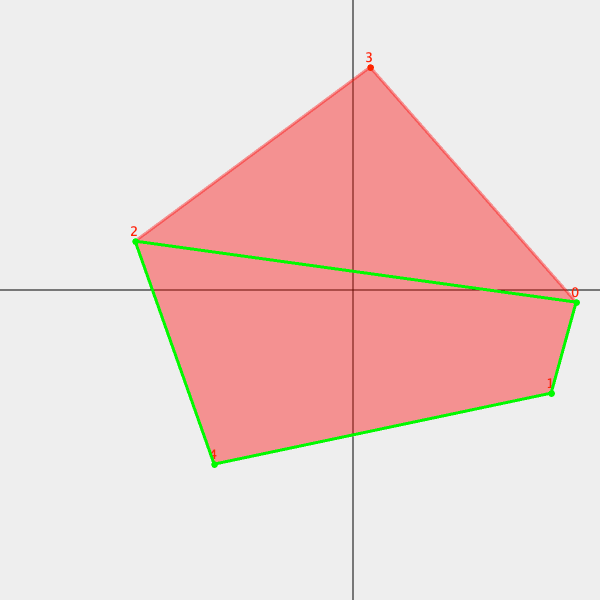
\includegraphics[width=0.3\textwidth]{media/CuttingSmallerAngle/5_4.png} &
        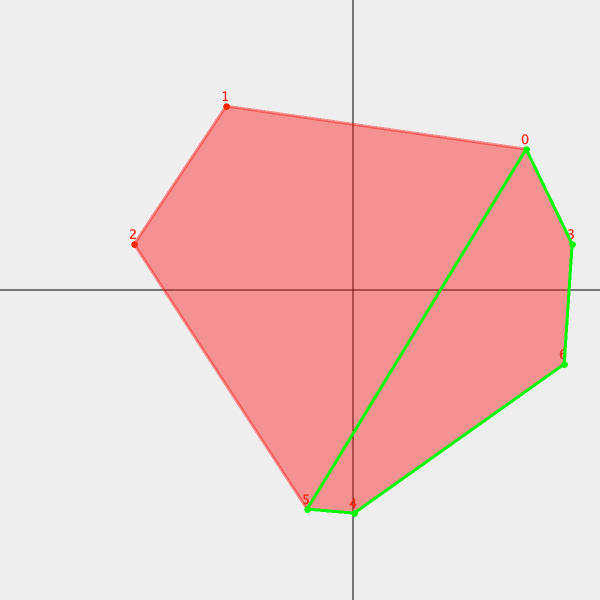
\includegraphics[width=0.3\textwidth]{media/CuttingSmallerAngle/7_5.png} &
        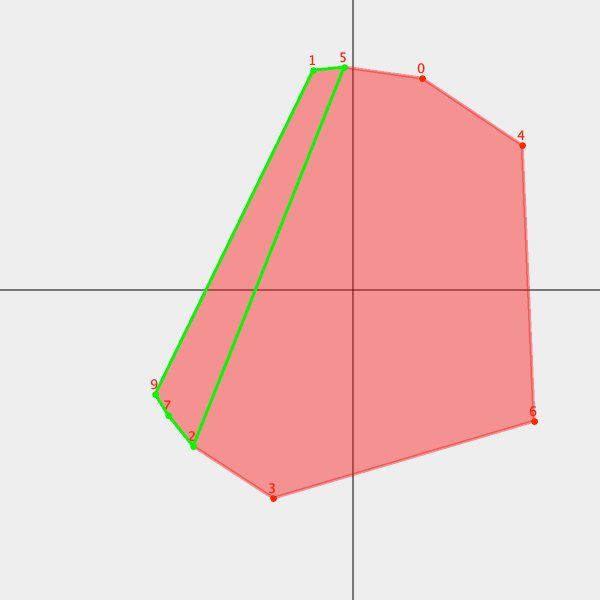
\includegraphics[width=0.3\textwidth]{media/CuttingSmallerAngle/9_5.png} \\
        (a) E = 5, h = 4 & (b) E = 7, h = 5 & (c) E = 9, h = 5
    \end{tabular}
\end{figure}

Le approssimazioni ottenute da questo algoritmo portano allo scarto di parti di regione ammissibili
poichè il politopo risultante sarà sempre una approssimazione per difetto dell'originale.

\pagebreak
\subsection{Ipotesi di Algoritmo Cutting Smaller Angle 2 (CSA2)}

Evolvendo la precedente ipotesi e consentendo all'algoritmo di poter includere i nodi esclusi 
da ciascun taglio traslando il suddetto, si può cosi creare un guscio che, oltre a essere 
convesso, rispetta l'inclusione di tutti i punti ammissibili.

\begin{figure}[H]
    \centering
    \begin{tabular}{c}
        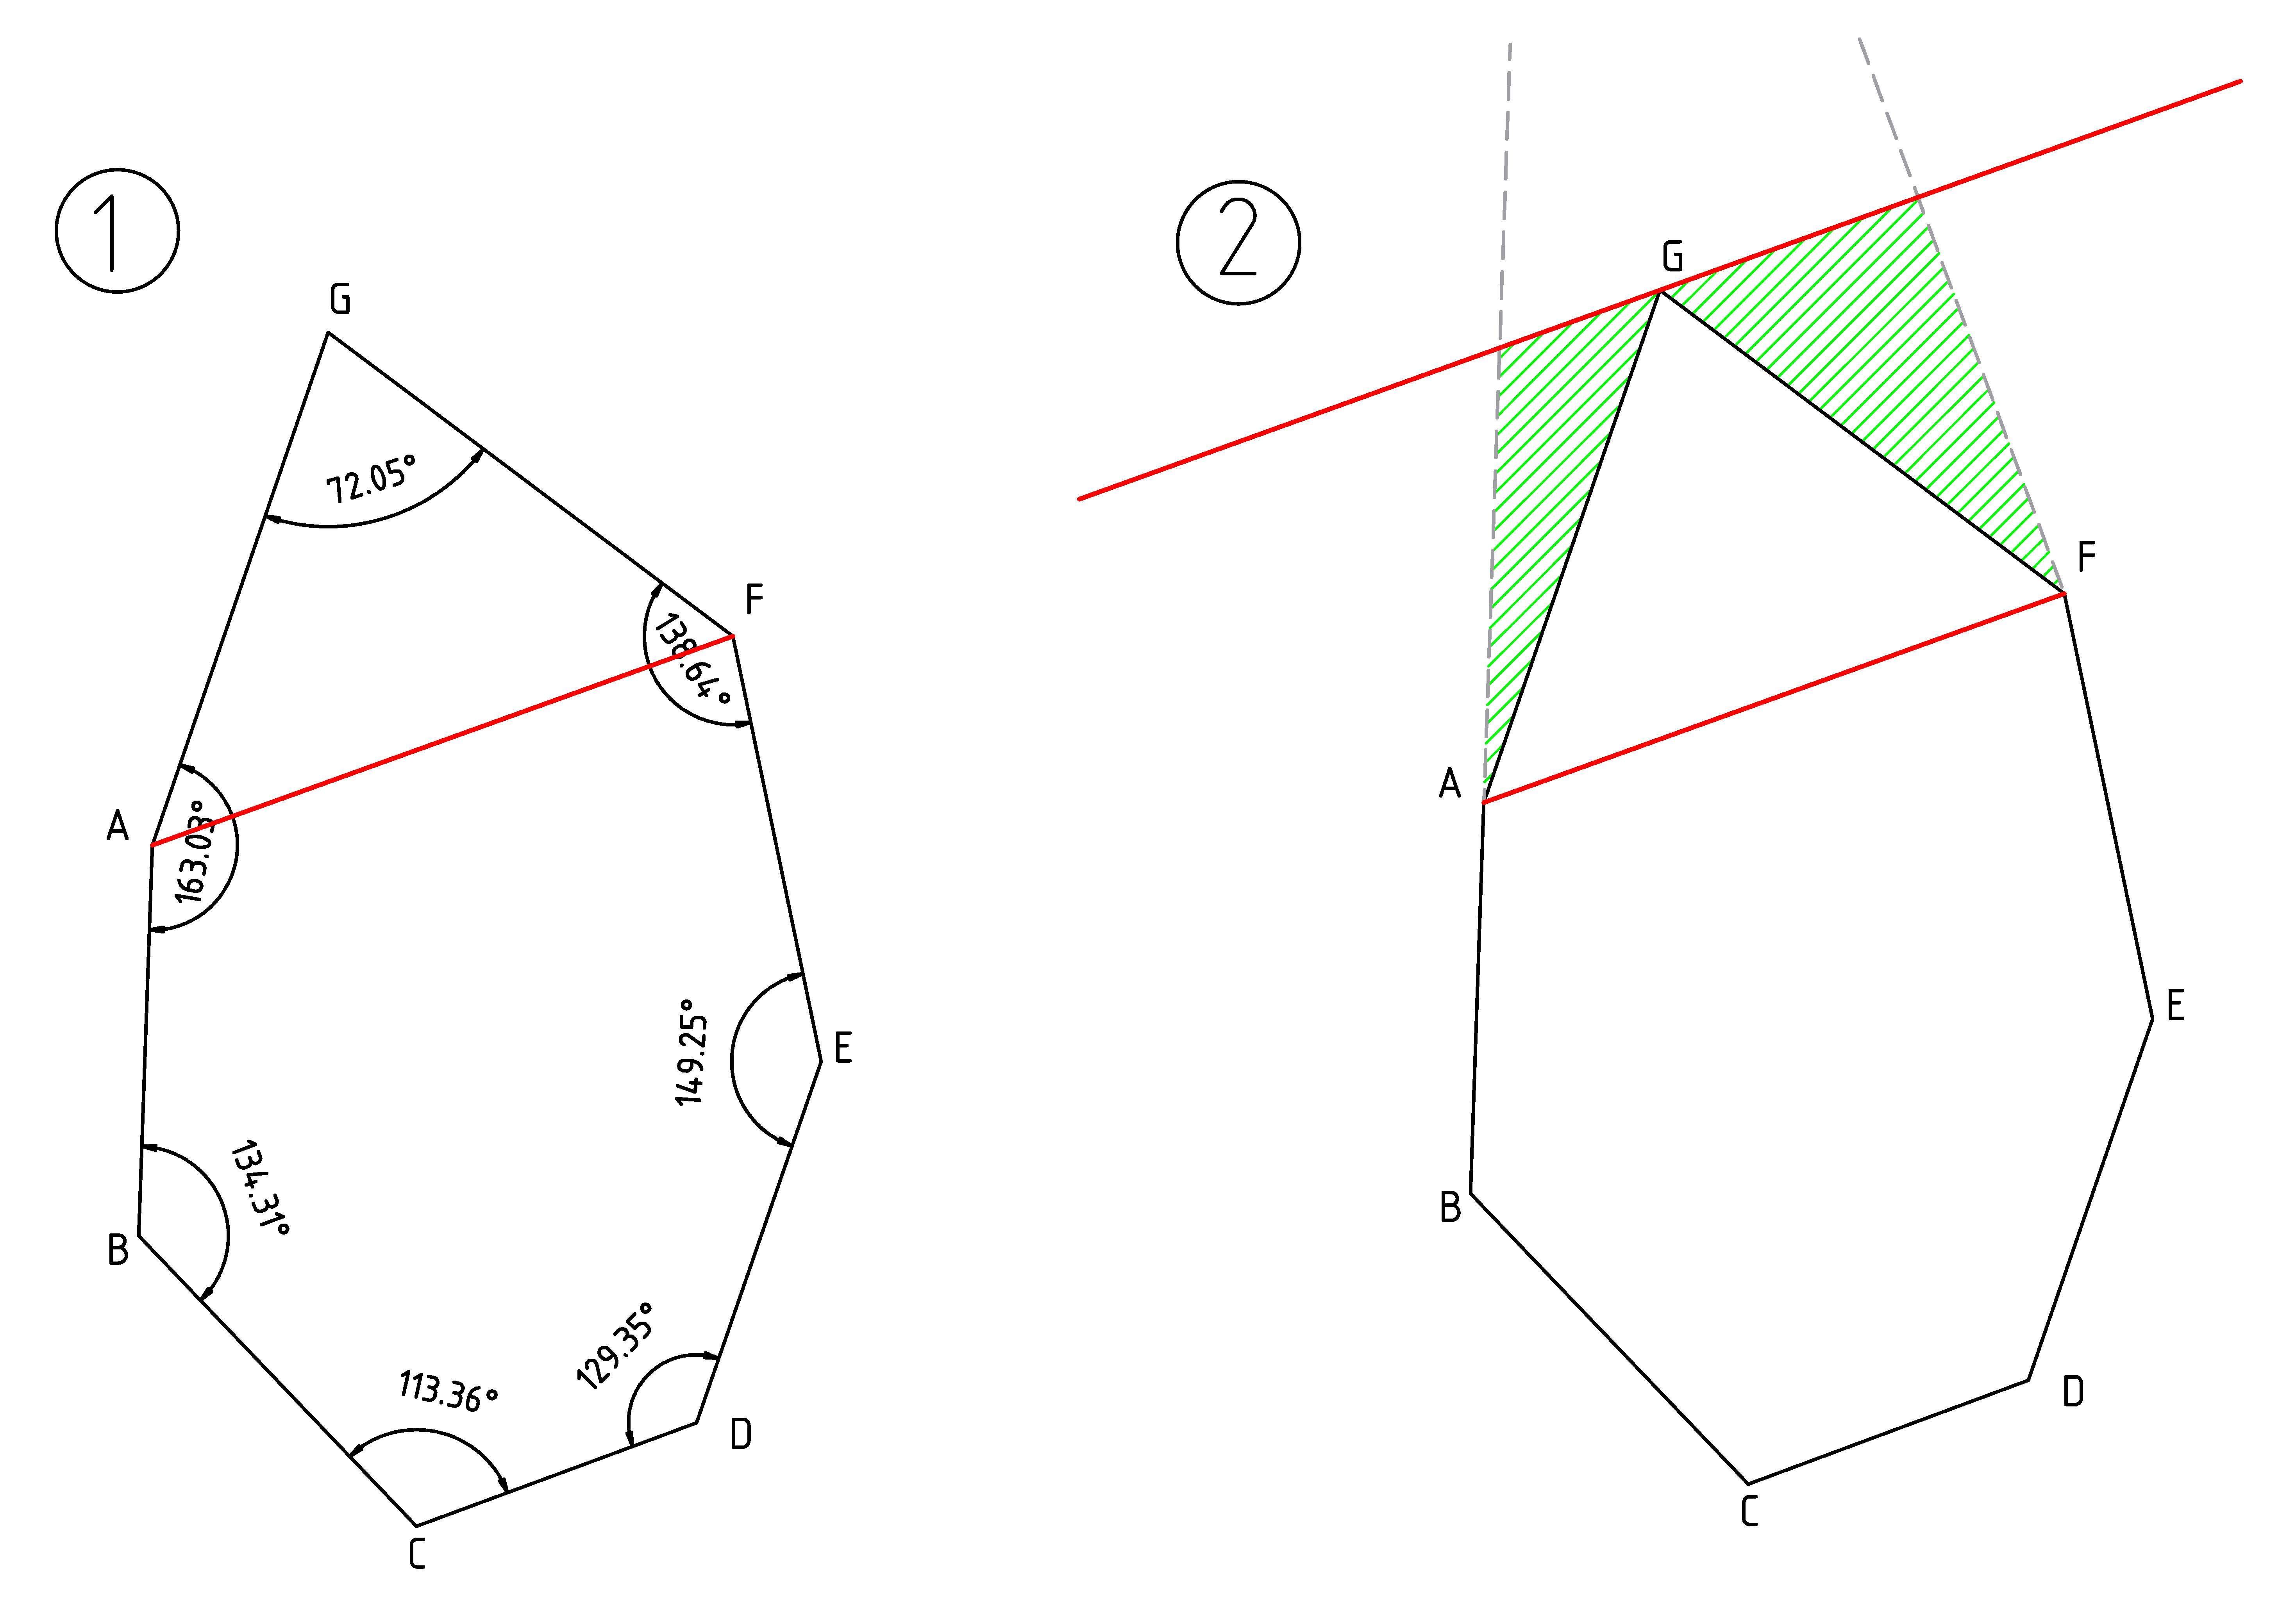
\includegraphics[width=0.8\textwidth]{media/Demo_algorithms/demo_smaller_angle.jpg} \\
        \begin{tabular}{l}
            (1) Creazione di un iperpiano secondo CSA \\
            (2) Traslazione dell'iperpiano creato secondo CSA2
        \end{tabular}
    \end{tabular}
\end{figure}

\begin{center}
    Esempi di approssimazione:
\end{center}
\begin{figure}[H]
    \centering
    \begin{tabular}{ccc}
        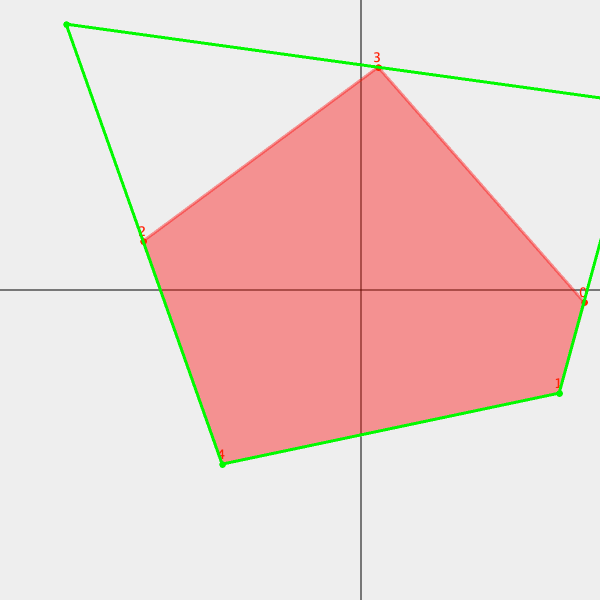
\includegraphics[width=0.3\textwidth]{media/CuttingSmallerAngle2/5_4.png} &
        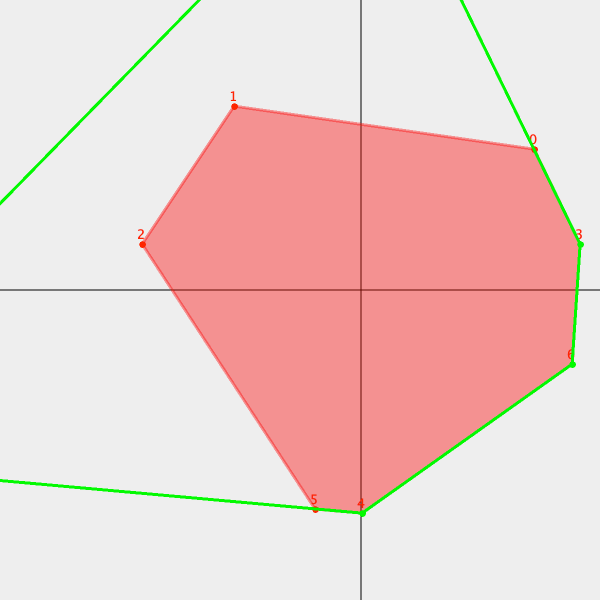
\includegraphics[width=0.3\textwidth]{media/CuttingSmallerAngle2/7_5.png} &
        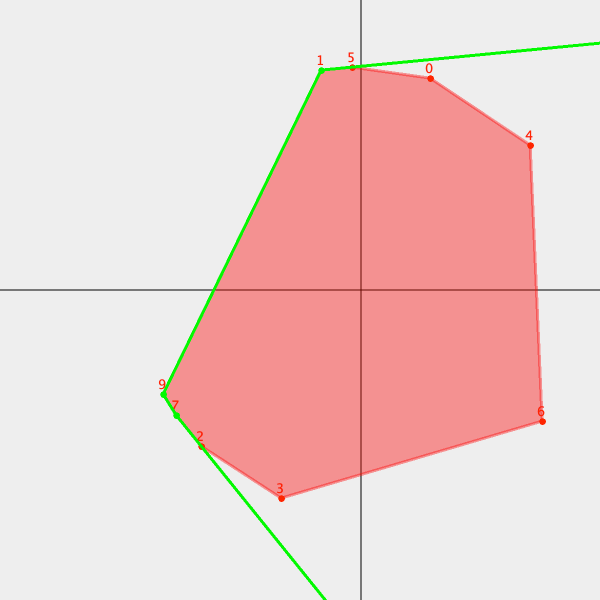
\includegraphics[width=0.3\textwidth]{media/CuttingSmallerAngle2/9_5.png} \\
        (a) E = 5, h = 4 & (b) E = 7, h = 5 & (c) E = 9, h = 5
    \end{tabular}
\end{figure}

Questo approccio rende l'algoritmo precedente accettabile poichè rispetta l'inclusione
dell'area ammissibile di partenza. Tuttavia, all'aumentare dei vertici, è molto probabile 
che un numero eccessivo di traslazioni interessino un iperpiano. questo porterebbe
alla deriva il lato rendendo, così il volume del politopo risultante eccessivo 
rispetto all'originale (come si può verificare dagli esempi (b) e (c)).


\pagebreak
\subsection{Ipotesi di Algoritmo Cutting Larger Angle (CLA)}

Utilizzando un approccio inverso all'algoritmo CSA, si potrebbe ipotizzare che gli angoli interni 
con ampiezza maggiore siano i candidati migliori per essere approssimati con un segmento, 
poichè la perdita di volume, una volta applicato il taglio, sarebbe la piu piccola possibile.

\begin{center}
    Esempi di approssimazione:
\end{center}
\begin{figure}[H]
    \centering
    \begin{tabular}{ccc}
        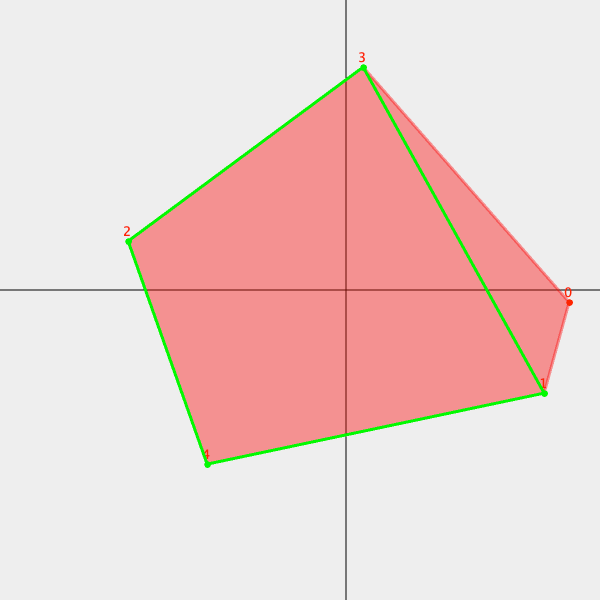
\includegraphics[width=0.3\textwidth]{media/CuttingLargerAngle/5_4.png} &
        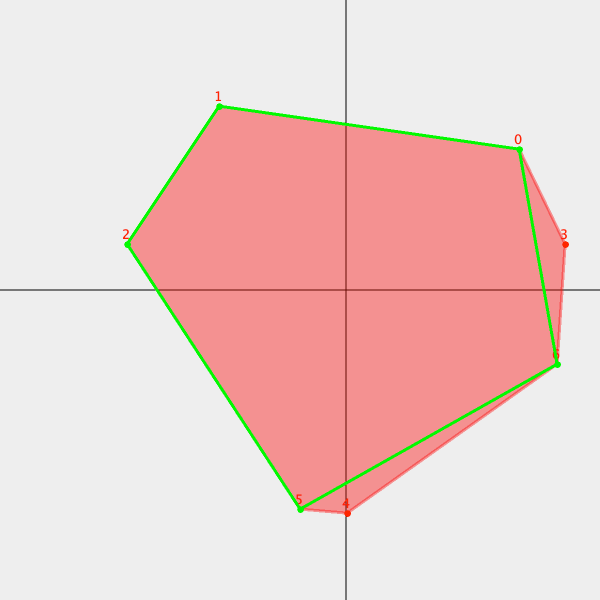
\includegraphics[width=0.3\textwidth]{media/CuttingLargerAngle/7_5.png} &
        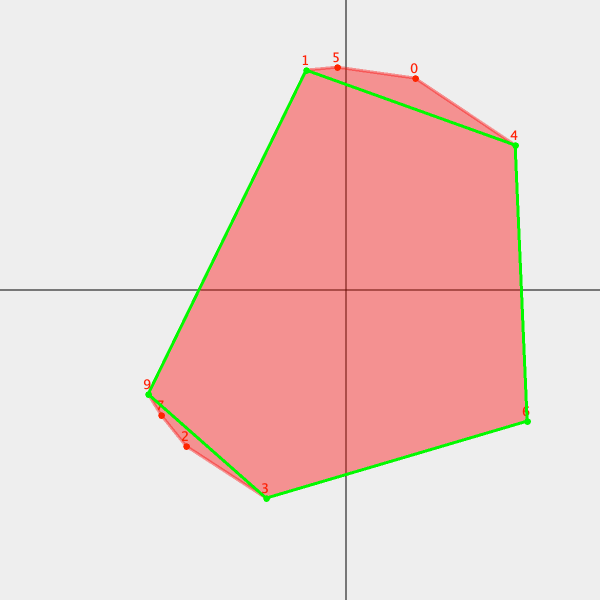
\includegraphics[width=0.3\textwidth]{media/CuttingLargerAngle/9_5.png} \\
        (a) E = 5, h = 4 & (b) E = 7, h = 5 & (c) E = 9, h = 5
    \end{tabular}
\end{figure}

Si rivela un approccio vincente in termini di somiglianza con l'area del guscio convesso di partenza, 
ma condivide con l'approccio CSA il fatto di non includere i nodi che vengono tagliati,
rendendolo così inaccettabile.

\pagebreak
\subsection{Ipotesi di Algoritmo Cutting Larger Angle 2 (CLA2)}

Applicando la medesima trasformazione applicata all'algoritmo CSA, si consente al precedente 
algoritmo di includere tutti i punti ammissibili, rendendo di fatto il precedente algoritmo accettabile.

\begin{figure}[H]
    \centering
    \begin{tabular}{c}
        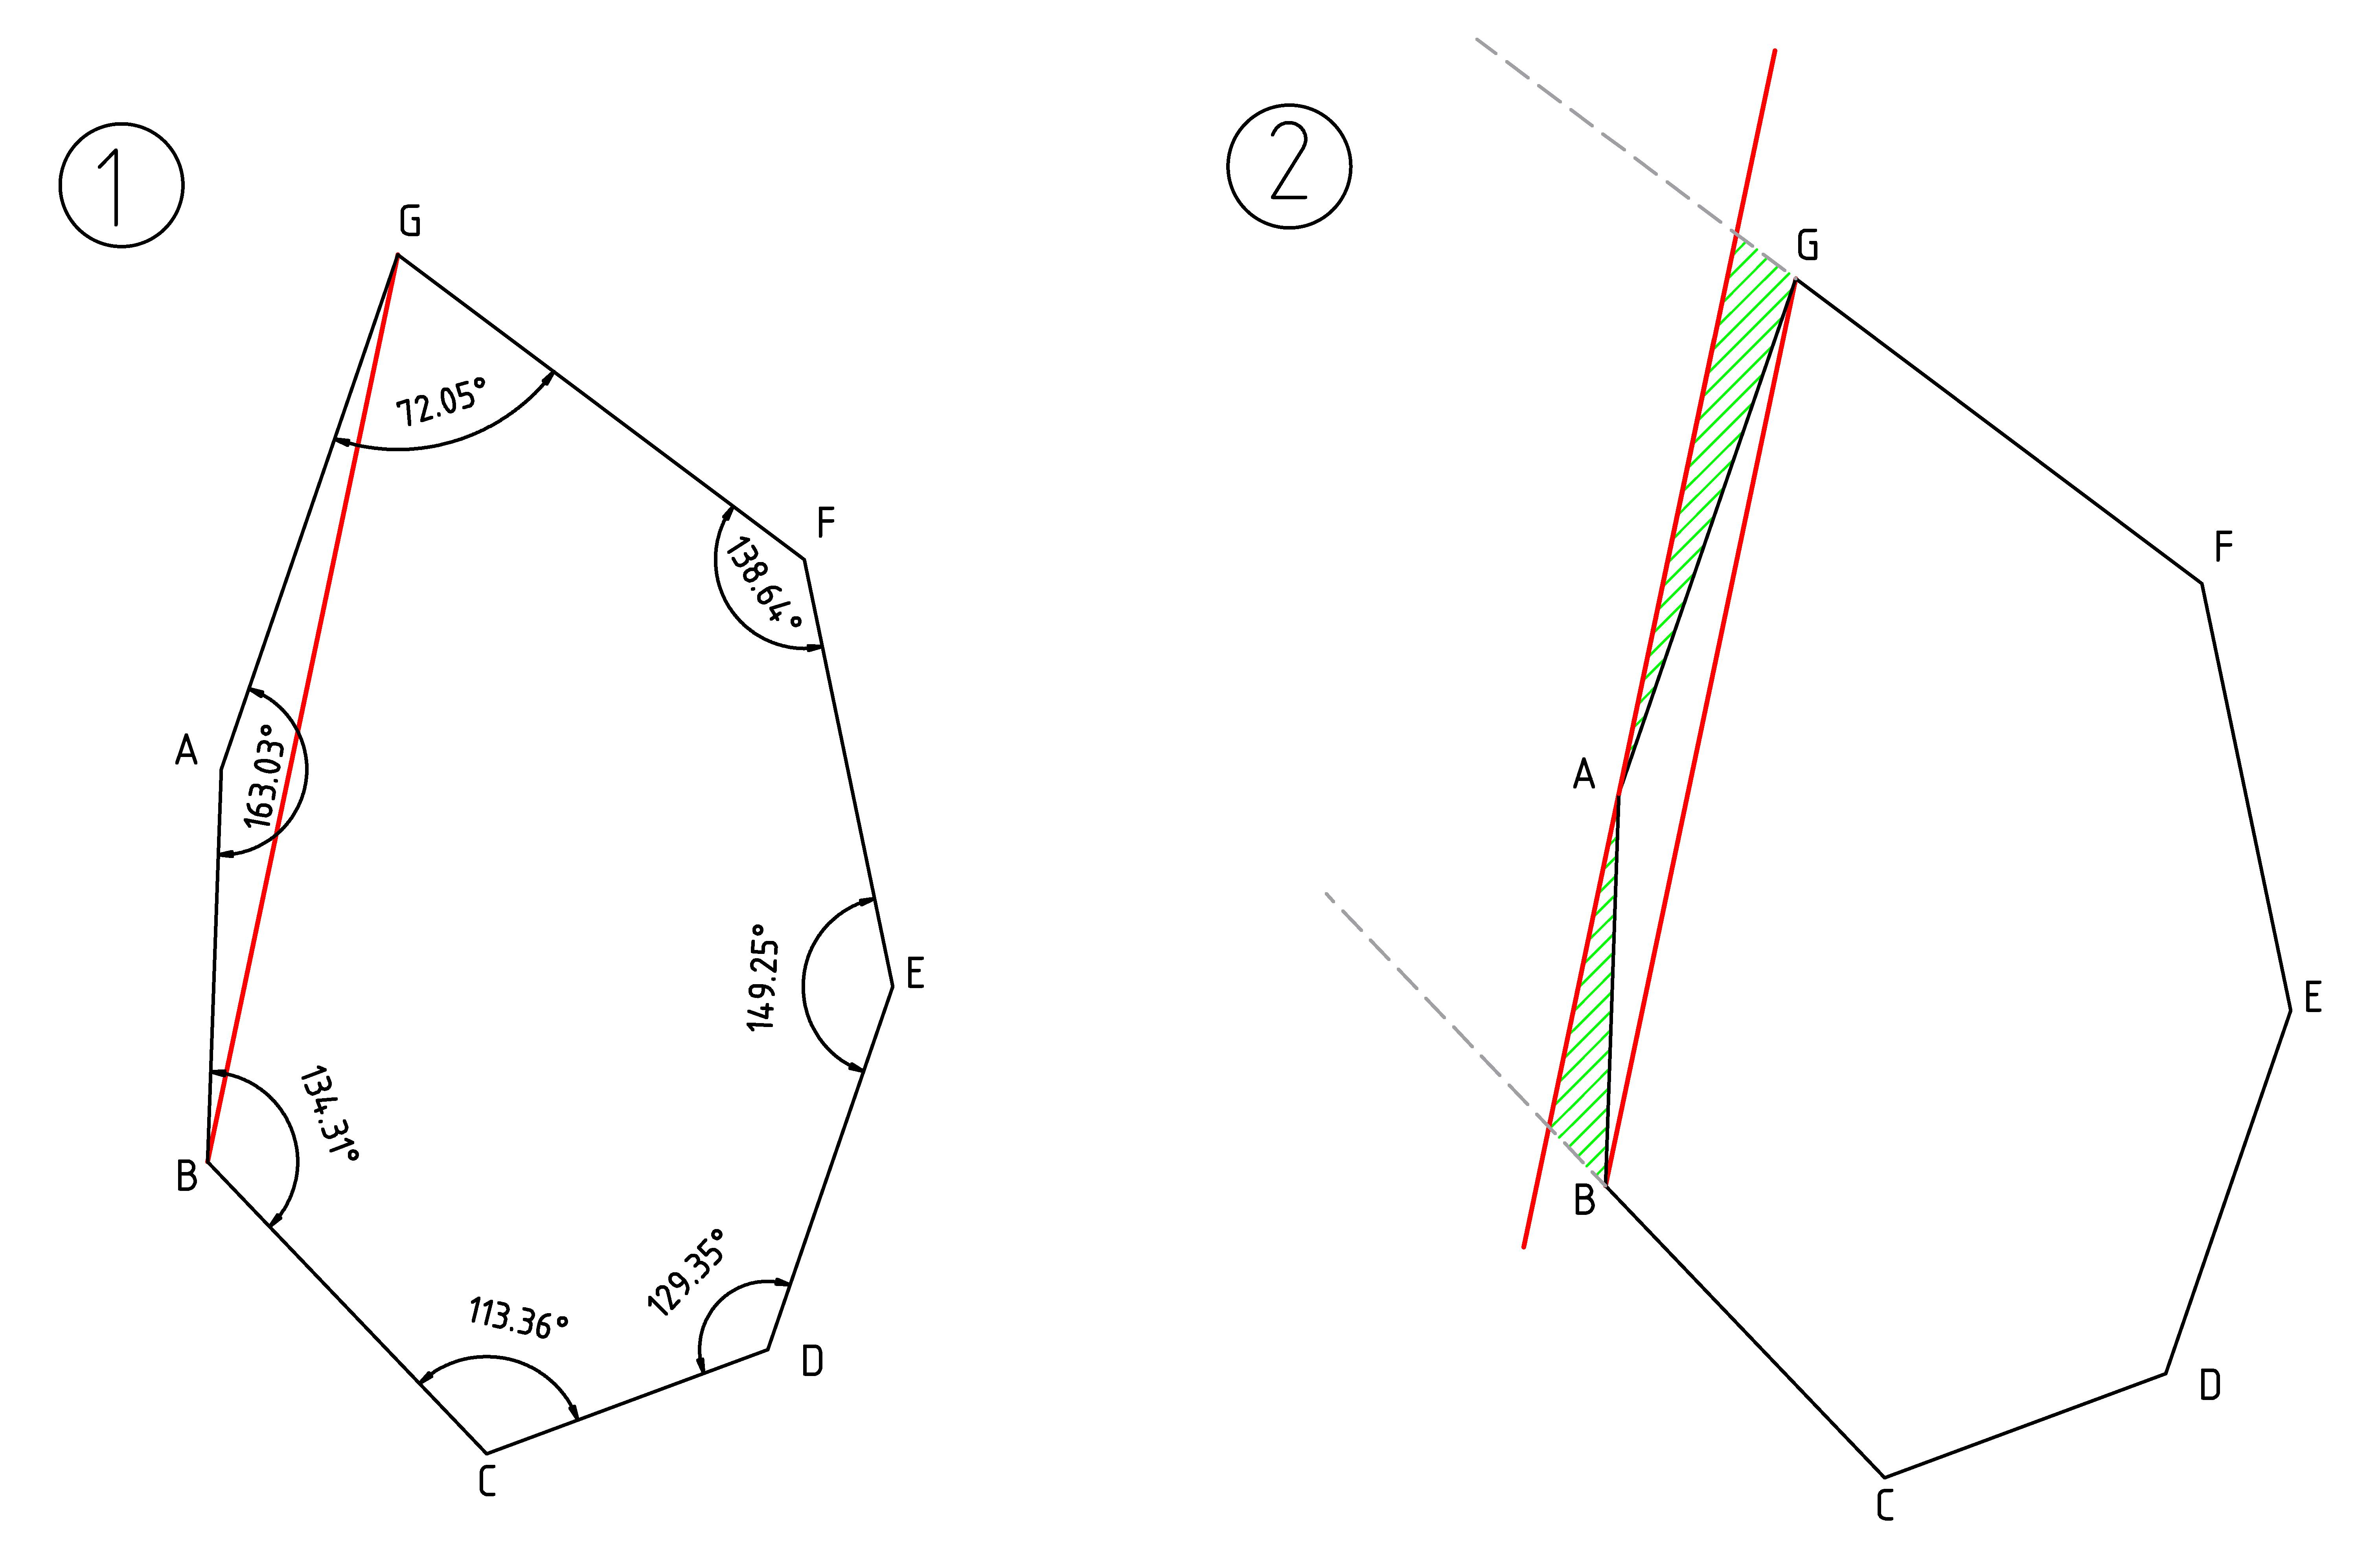
\includegraphics[width=0.8\textwidth]{media/Demo_algorithms/demo_larger_angle.jpg} \\
        \begin{tabular}{l}
            (1) Creazione di un iperpiano secondo CLA \\
            (2) Traslazione dell'iperpiano creato secondo CLA2
        \end{tabular}
    \end{tabular}
\end{figure}

\begin{center}
    Esempi di approssimazione:
\end{center}
\begin{figure}[H]
    \centering
    \begin{tabular}{ccc}
        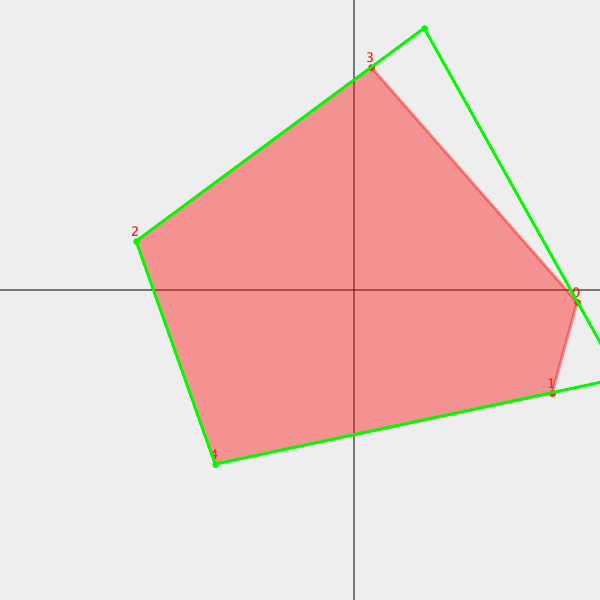
\includegraphics[width=0.3\textwidth]{media/CuttingLargerAngle2/5_4.png} &
        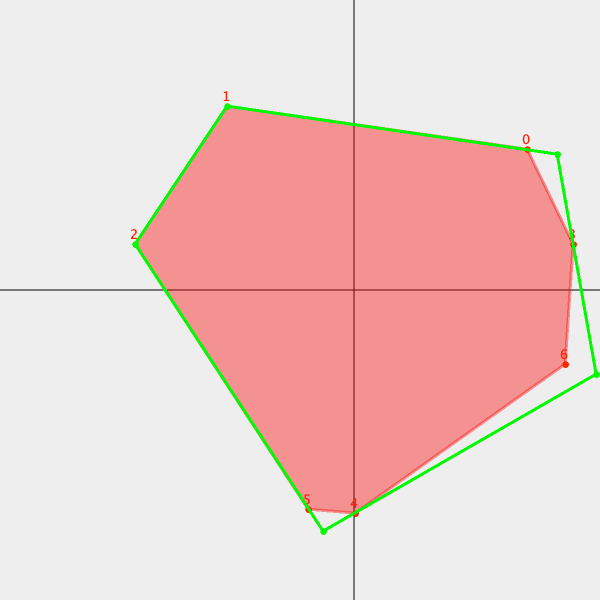
\includegraphics[width=0.3\textwidth]{media/CuttingLargerAngle2/7_5.png} &
        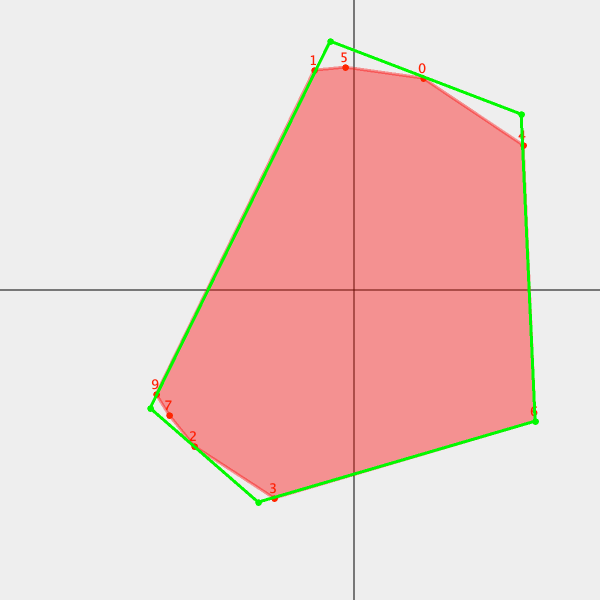
\includegraphics[width=0.3\textwidth]{media/CuttingLargerAngle2/9_5.png} \\
        (a) e = 5, h = 4 & (b) e = 7, h = 5 & (c) e = 9, h = 5
    \end{tabular}
\end{figure}

Il risultato ottenuto, in termini di somiglianza visiva con il poligono originale, è buono. 
A rafforzare questo punto viene anche il rispettivo indice di Jaccard analizzato nella sezione 
\hyperref[sec:Analisi dei dati]{Analisi dei dati}.

\pagebreak
\subsection{Ipotesi di Algoritmo Distance From G (DFG)}

Questo algoritmo prevede la ricerca dei vertici più distanti dal baricentro del guscio convesso. 
Una volta selezionati $h$ vertici, viene costruito il poligono risultante.
Successivamente ogni lato che esclude vertici del poliedro originale viene traslato fino al 
loro contenimento.\\

Onde evitare che un numero elevato di vertici concentrati in una regione limitata del guscio convesso
influenzino il calcolo del baricentro calcolato con la formula 
\[
G_i = \frac{1}{n} \sum_{k=1}^{n} x_{k,i}
\]
si procede a considerare come baricentro della regione ammissibile il centro di massa 
della corrispettiva \textit{bounding box}.\\

\begin{figure}[H]
    \centering
    \begin{tabular}{c}
        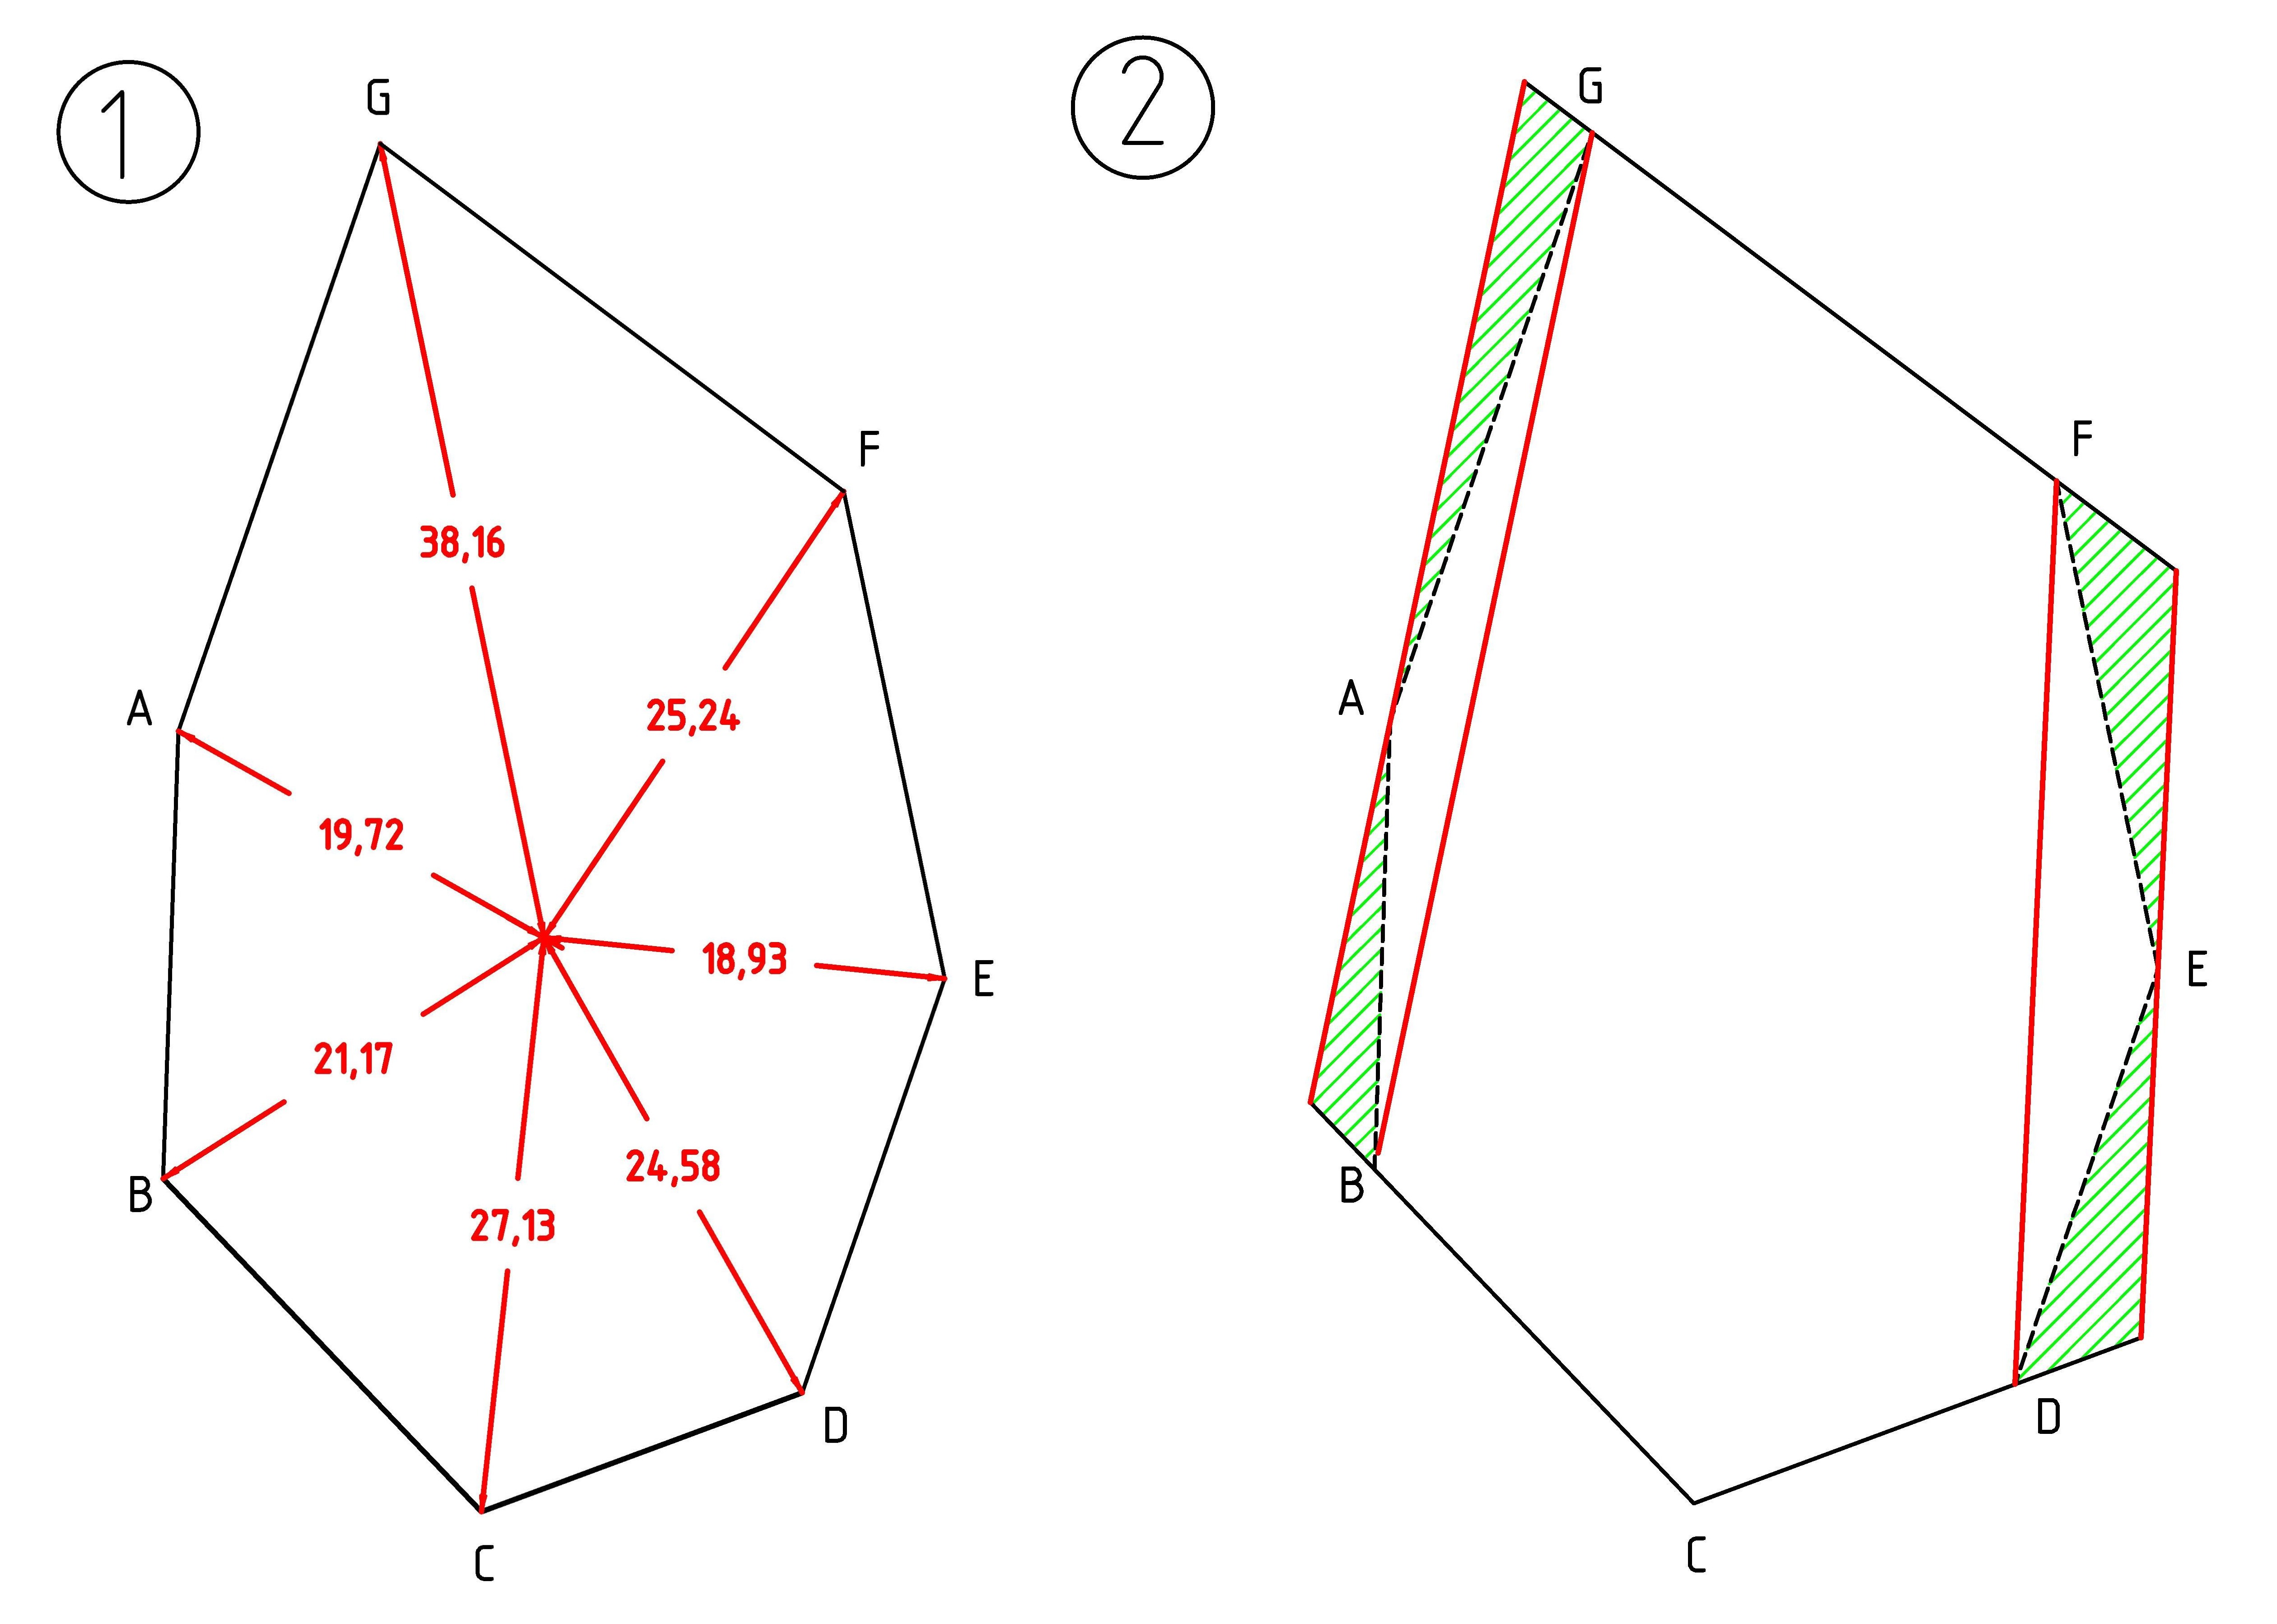
\includegraphics[width=0.8\textwidth]{media/Demo_algorithms/demo_distance_g.jpg} \\
        \begin{tabular}{l}
            (1) Dimostrazione del criterio di scelta dei vertici secondo DFG\\
            (2) Traslazione degli iperpiani interni dell'approssimazione secondo DFG
        \end{tabular}
    \end{tabular}
\end{figure}

\begin{center}
    Esempi di approssimazione:
\end{center}
\begin{figure}[H]
    \centering
    \begin{tabular}{ccc}
        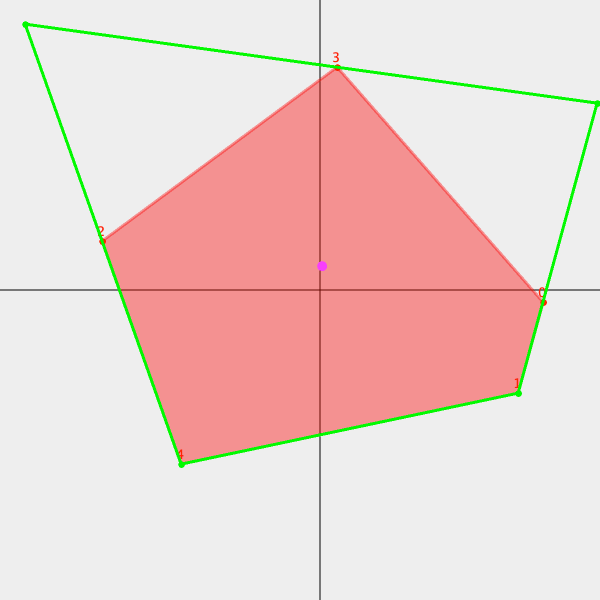
\includegraphics[width=0.3\textwidth]{media/DistanceFromG/5_4.png} &
        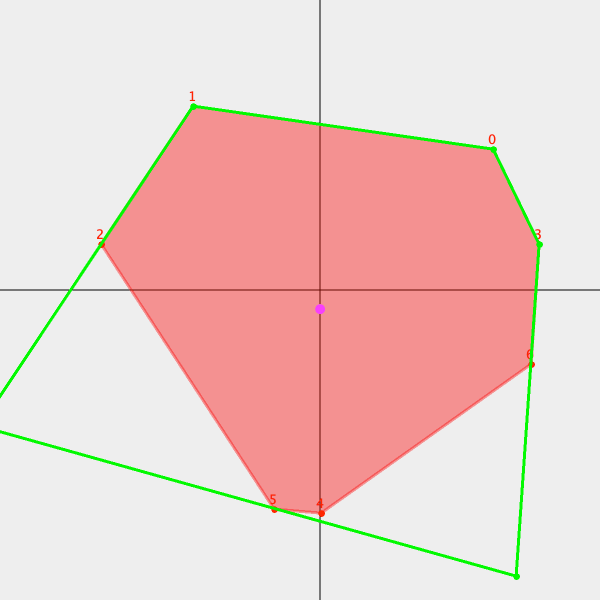
\includegraphics[width=0.3\textwidth]{media/DistanceFromG/7_5.png} &
        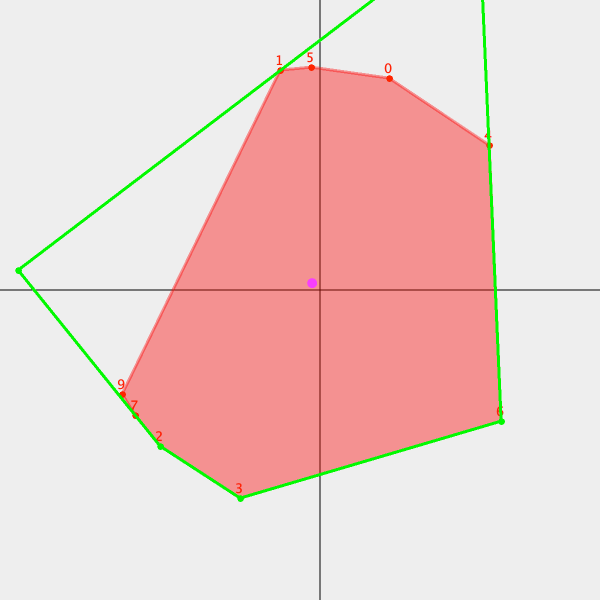
\includegraphics[width=0.3\textwidth]{media/DistanceFromG/9_5.png} \\
        (a) E = 5, h = 4 & (b) E = 7, h = 5 & (c) E = 9, h = 5
    \end{tabular}
\end{figure}

\pagebreak
\section{Approssimazioni tramite analisi delle proprietà degli iperpiani}

A differenza dei precedenti, gli algoritmi illustrati di seguito analizzano proprietà
intrinseche degli iperpiani del guscio convesso (come volumi eccedenti o aree proiettate),
selezionando un numero di iperpiani congruo al budget fornito secondo differenti criteri.
Questa caratteristica garantisce che, in un qualunque passaggio di computazione, 
il politopo approssimativo non escluda mai parti della regione ammissibile di partenza.

\subsection{Ipotesi di Algoritmo BoxCutting}

L'algoritmo prende direttamente in considerazione la \textit{Bounding Box} del 
politopo originale per poter effettuare dei tagli al volume di questa in modo tale 
che, con ognuno di questi, il volume generato dagli iperpiani di taglio arrivi a 
combaciare con quello originale.
Per sua natura utilizza un approccio inverso agli altri algoritmi della categoria 
poichè, a partire da un poliedro più semplice, si converge verso il politopo originale.

\begin{figure}[H]
    \centering
    \begin{tabular}{c}
        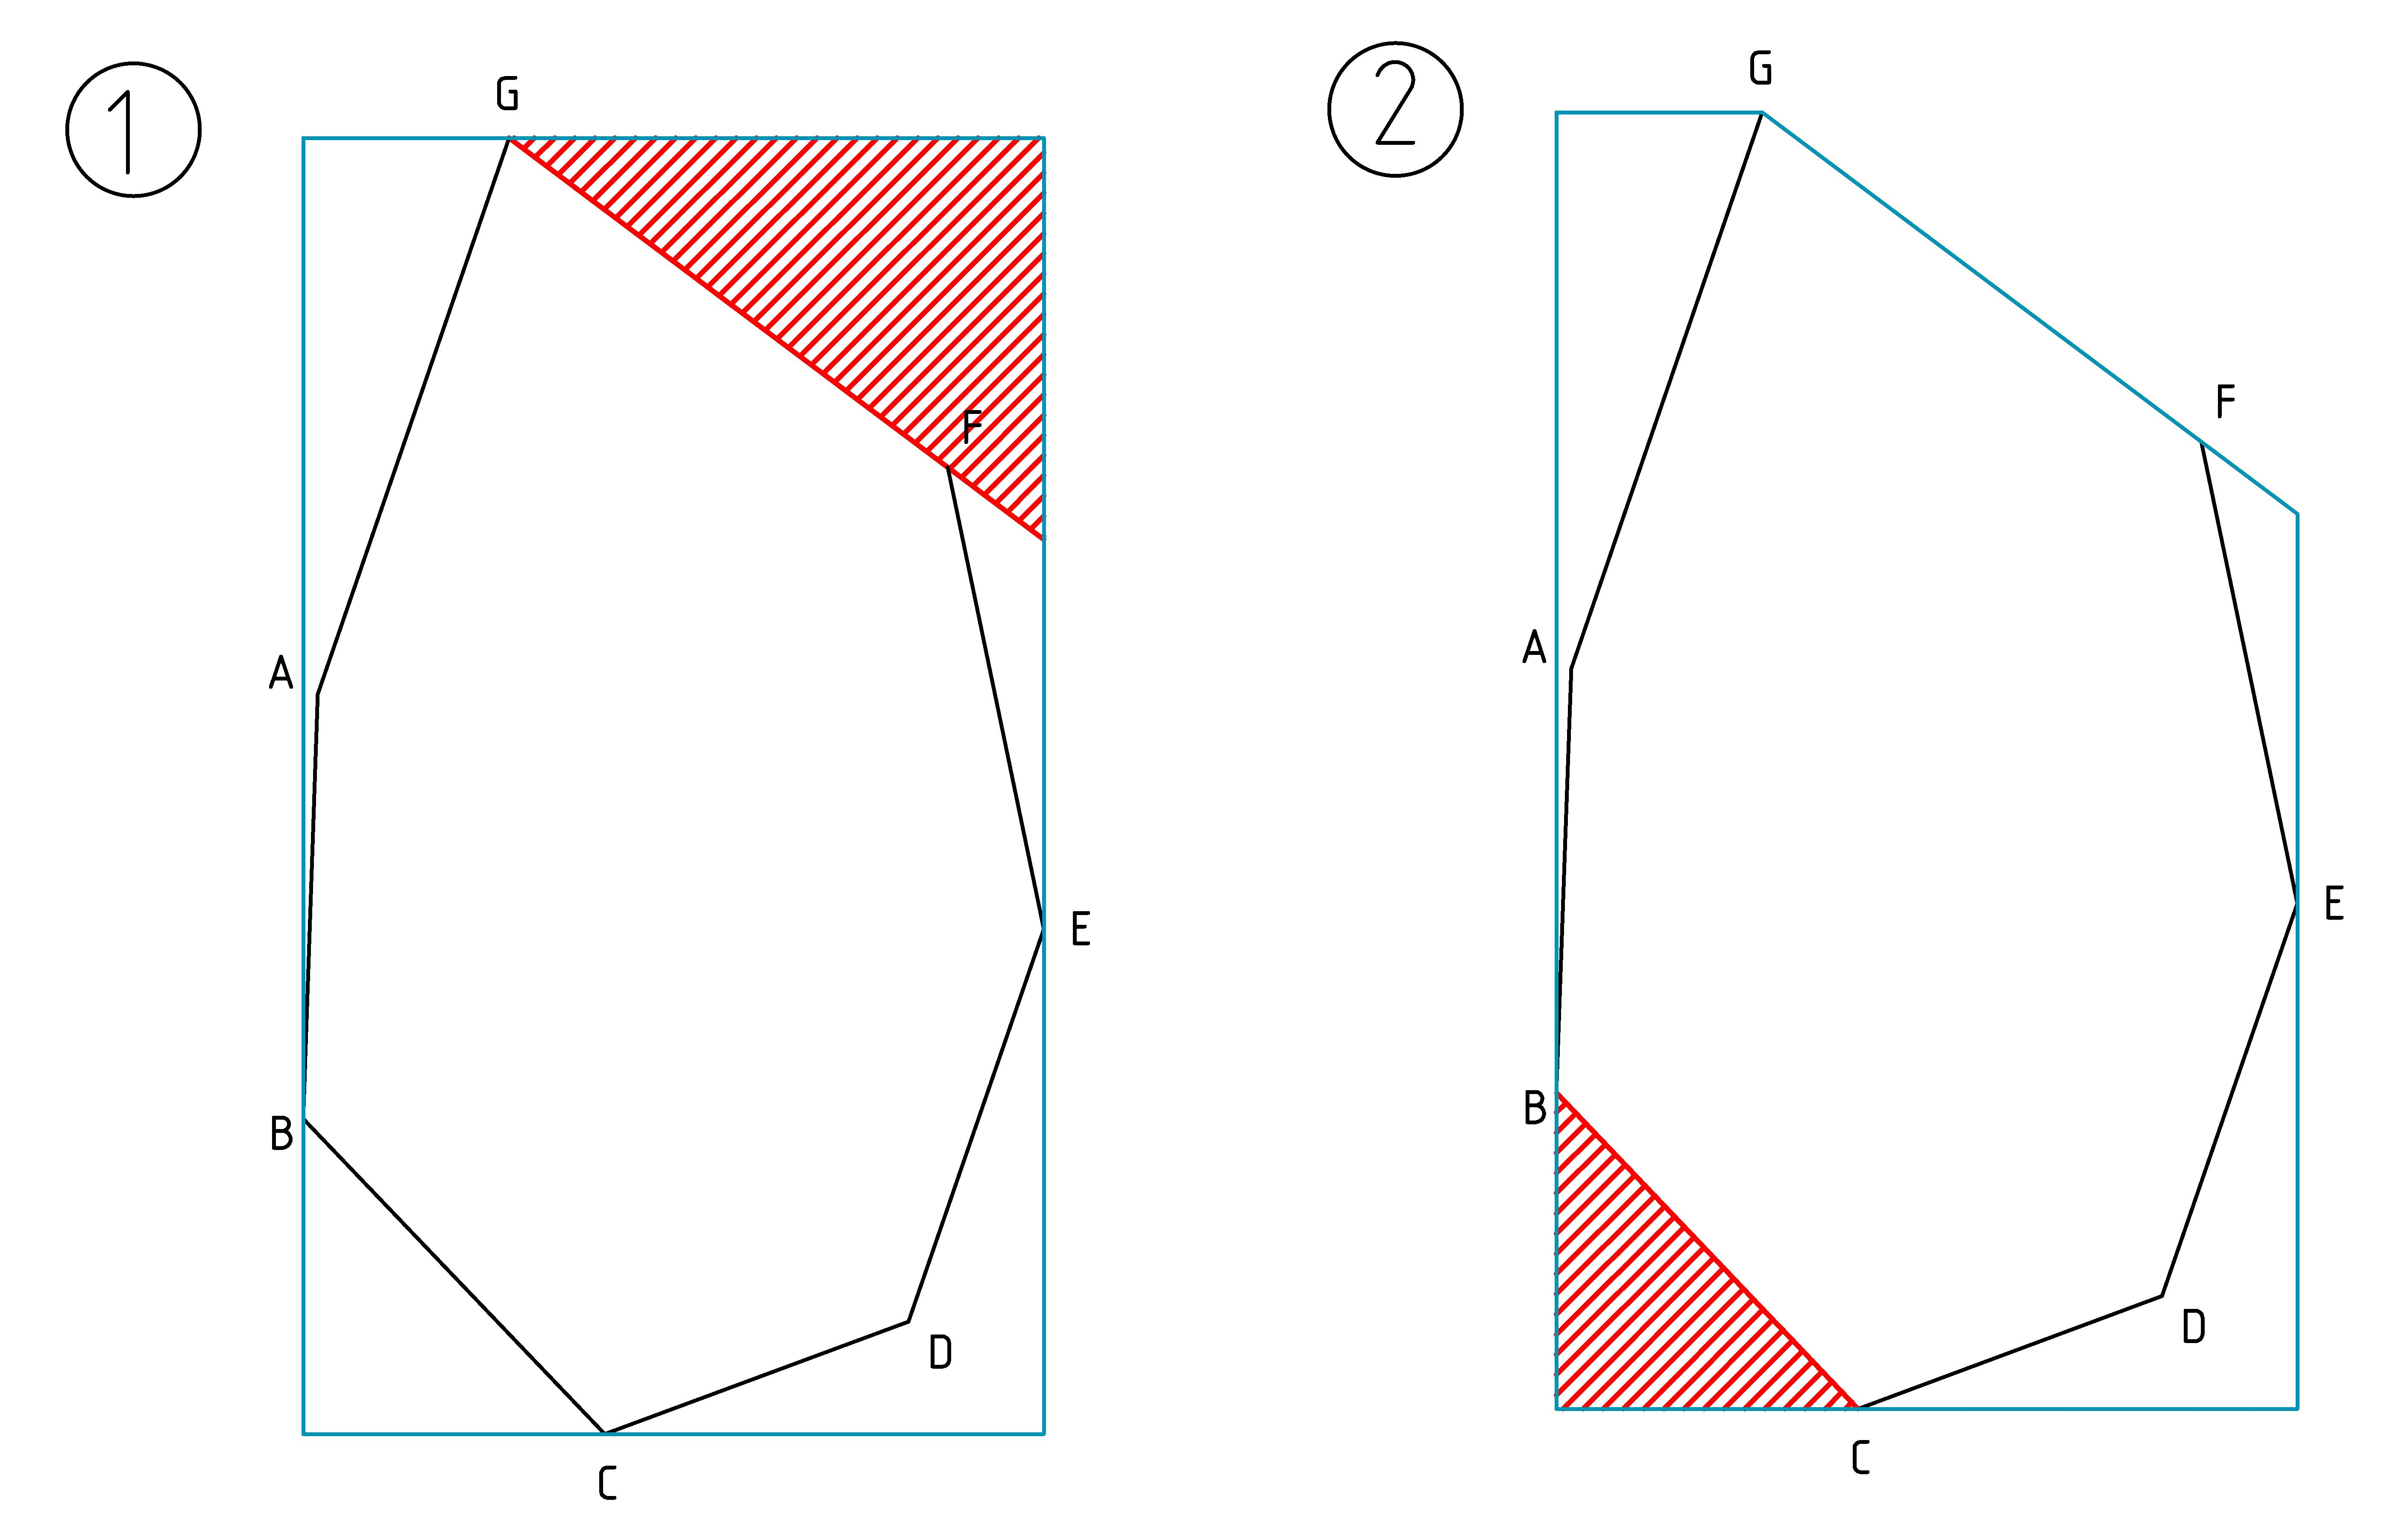
\includegraphics[width=0.8\textwidth]{media/Demo_algorithms/demo_box_cutting.jpg} \\
        \begin{tabular}{l}
            (1) Dimostrazione del criterio di scelta dell'iperpiano migliore secondo B.C.\\
            (2) Dimostrazione del criterio di scelta sul restante politopo
        \end{tabular}
    \end{tabular}
\end{figure}

\begin{center}
    Esempi di approssimazione:
\end{center}
\begin{figure}[H]
    \centering
    \begin{tabular}{ccc}
        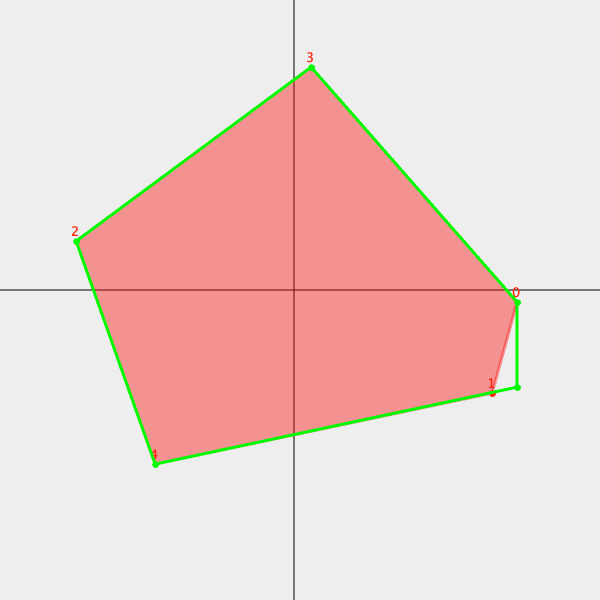
\includegraphics[width=0.3\textwidth]{media/BoxCutting/5_4.png} &
        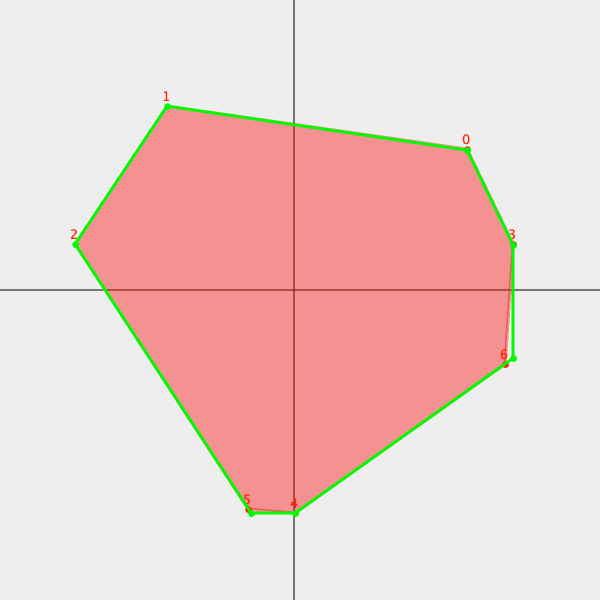
\includegraphics[width=0.3\textwidth]{media/BoxCutting/7_5.png} &
        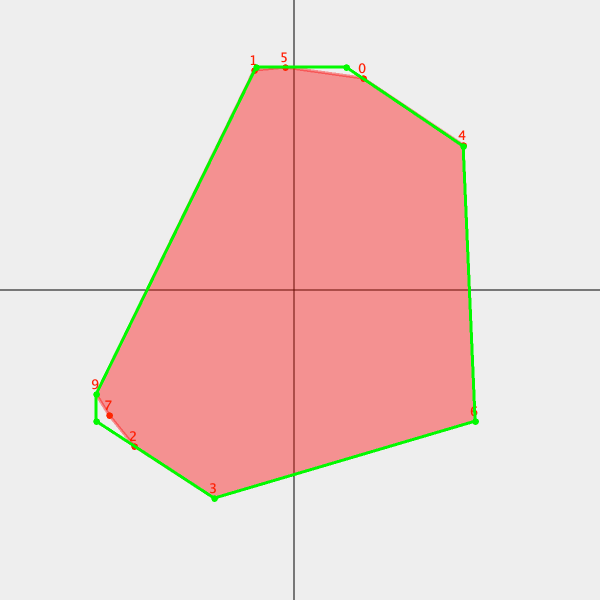
\includegraphics[width=0.3\textwidth]{media/BoxCutting/9_5.png} \\
        (a) E = 5, h = 4 & (b) E = 7, h = 5 & (c) E = 9, h = 5
    \end{tabular}
\end{figure}

L'approccio unico utilizzato offre diversi vantaggi, quali l'ottenimento di una approssimazione
con pochi iperpiani del politopo originale sin dalle prime iterazioni.
L'approssimazione diventa di fatti progressivamente costosa computazionalmente al crescere
di $h$.


\subsection{Ipotesi di Algoritmo Less Area}

L'algoritmo ipotizzato cerca i lati che meglio possano rappresentare un lato del poligono 
selezionando gli iperpiani che tendono a minimizzare l'area compresa fra essi e il poligono stesso, 
come mostrato in figura.

\begin{figure}[H]
    \centering
    \begin{tabular}{c}
        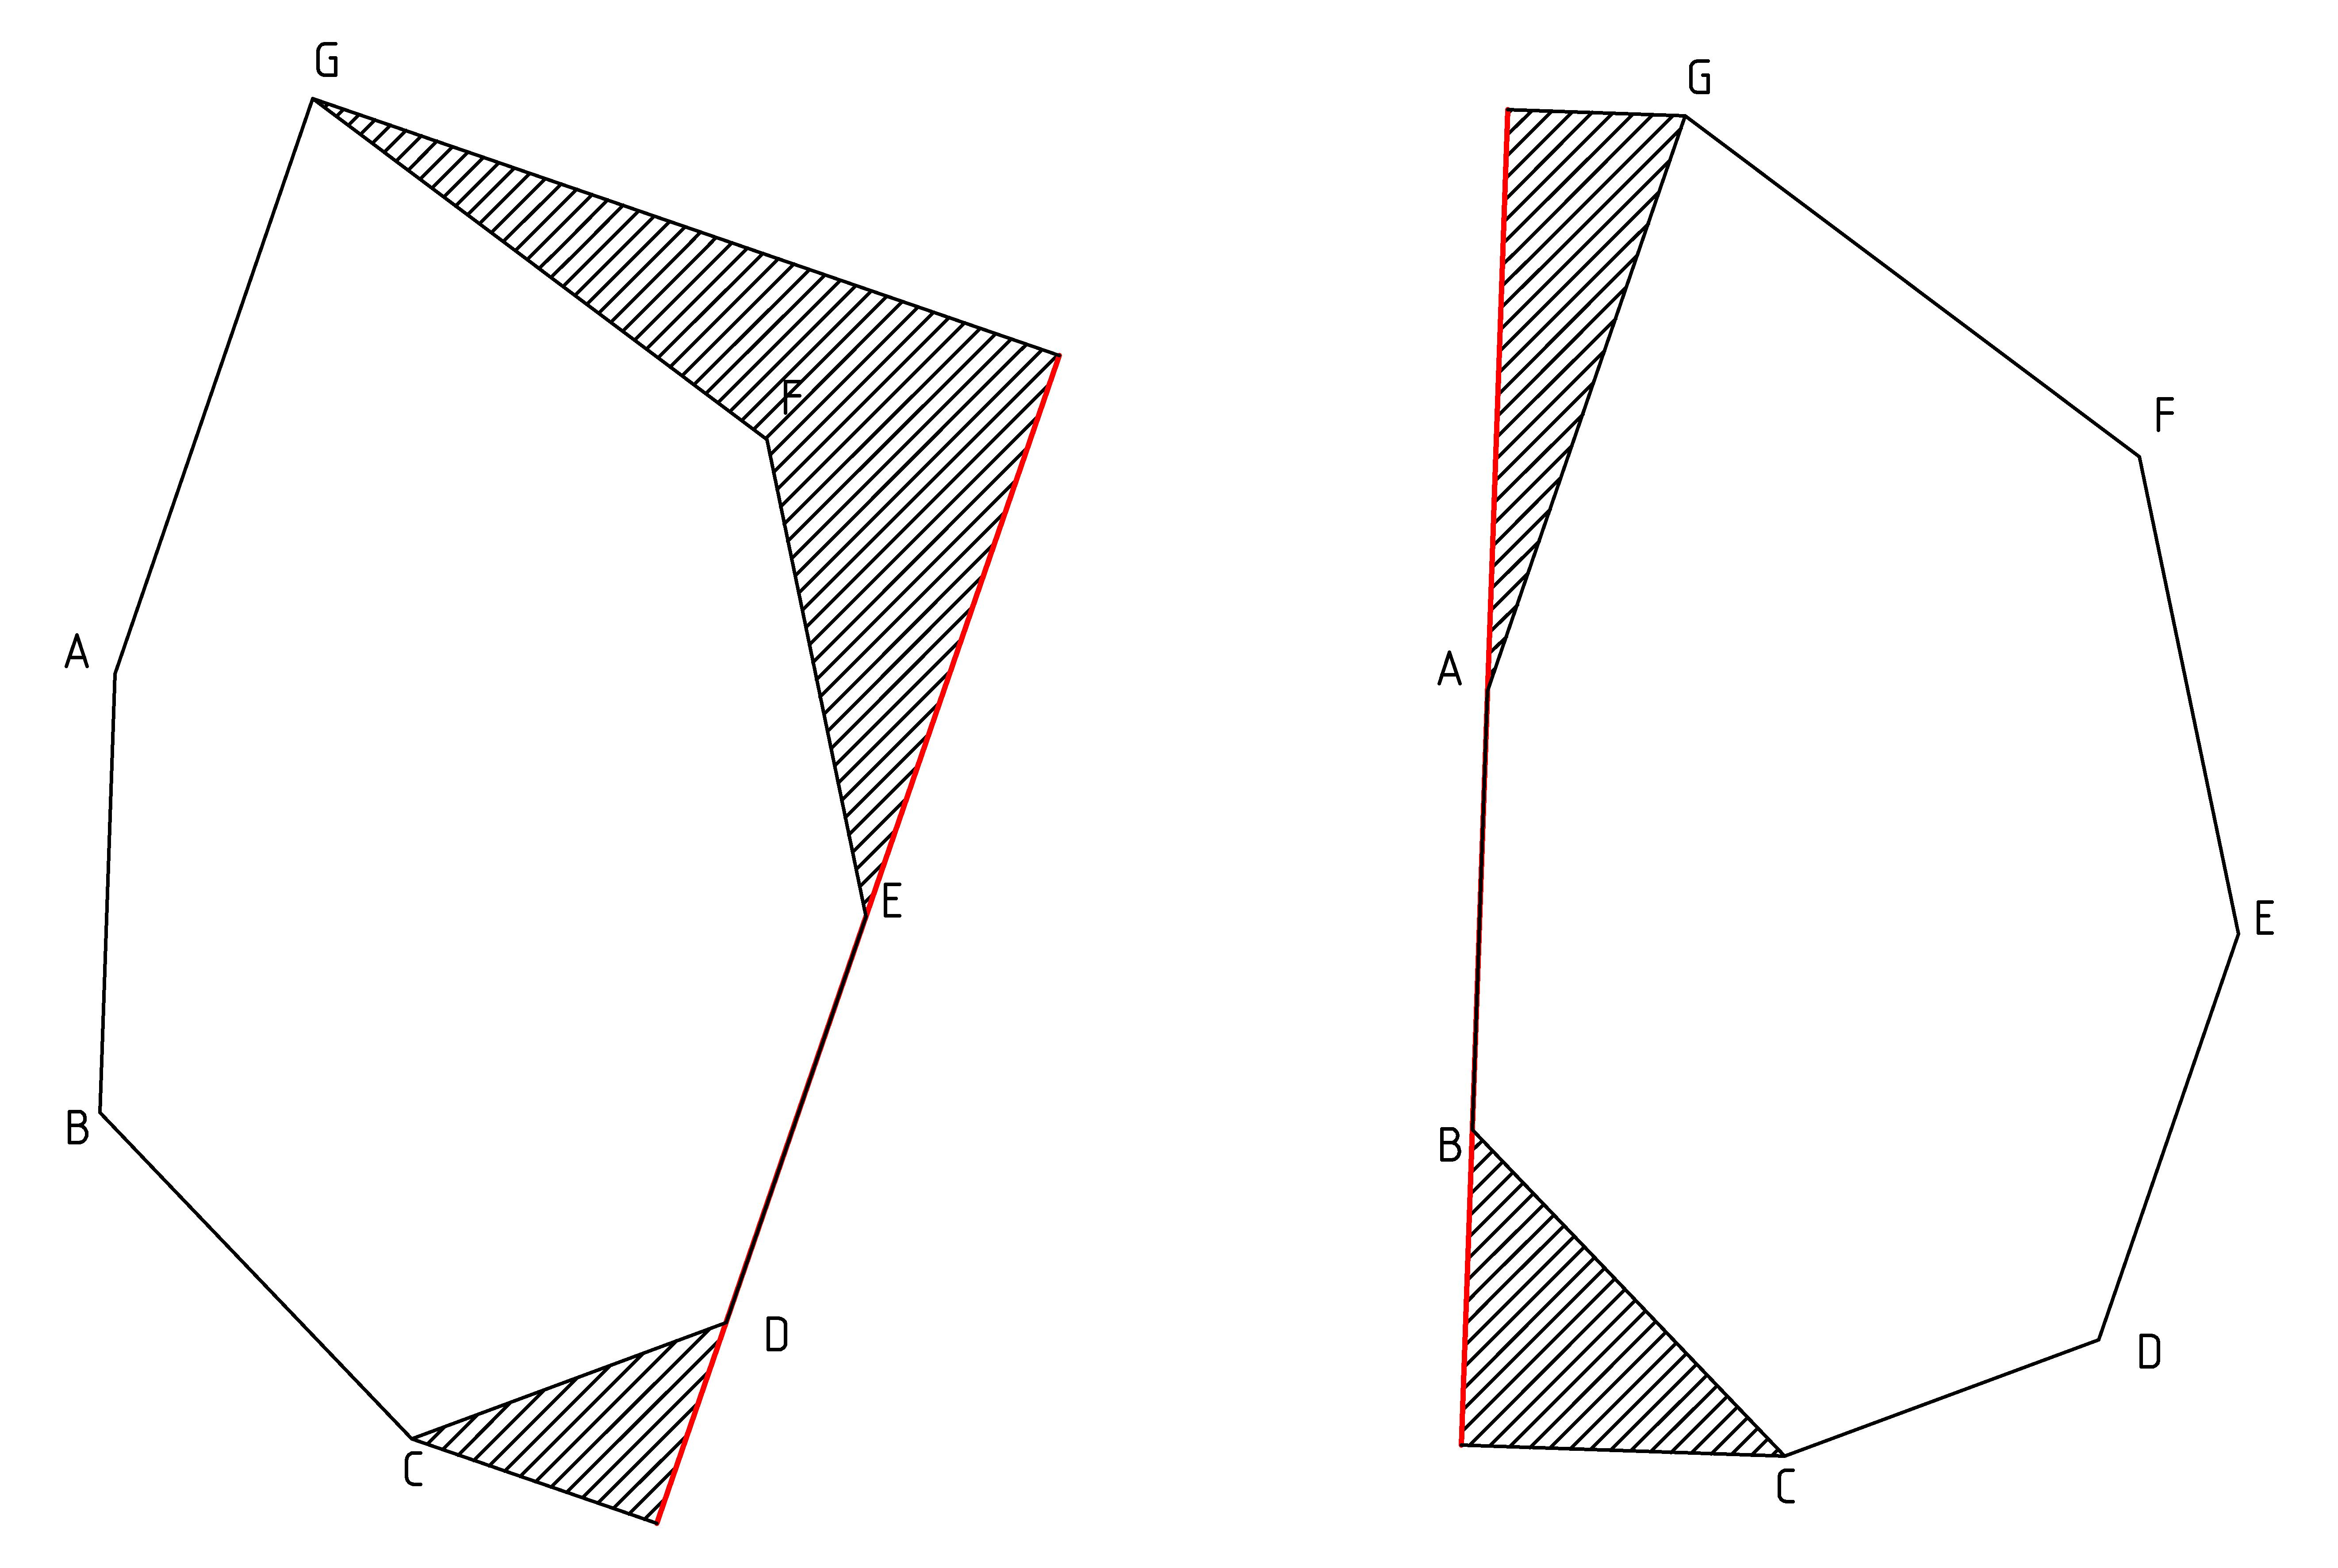
\includegraphics[width=0.8\textwidth]{media/Demo_algorithms/demo_smaller_area.jpg} \\
        \begin{tabular}{l}
            Dimostrazione del criterio di ordinamento degli iperpiani\\
        \end{tabular}
    \end{tabular}
\end{figure}

\begin{center}
    Esempi di approssimazione:
\end{center}
\begin{figure}[H]
    \centering
    \begin{tabular}{ccc}
        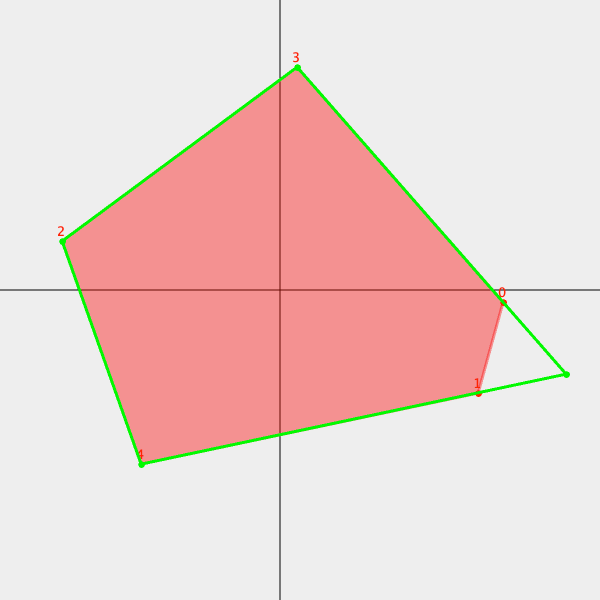
\includegraphics[width=0.3\textwidth]{media/LessArea/5_4.png} &
        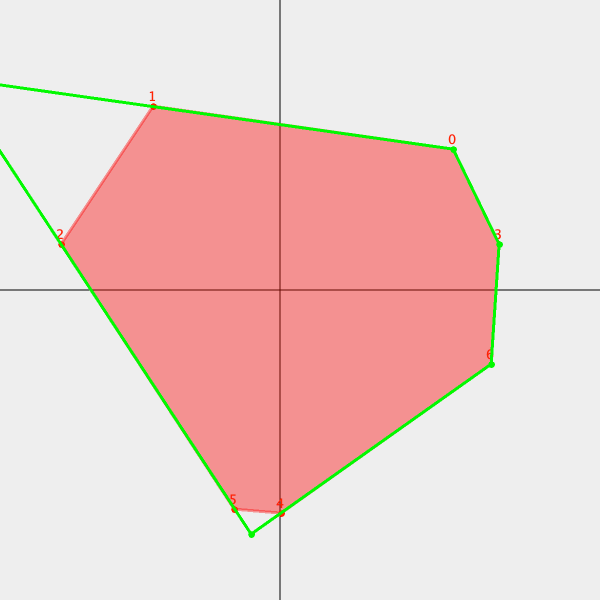
\includegraphics[width=0.3\textwidth]{media/LessArea/7_5.png} &
        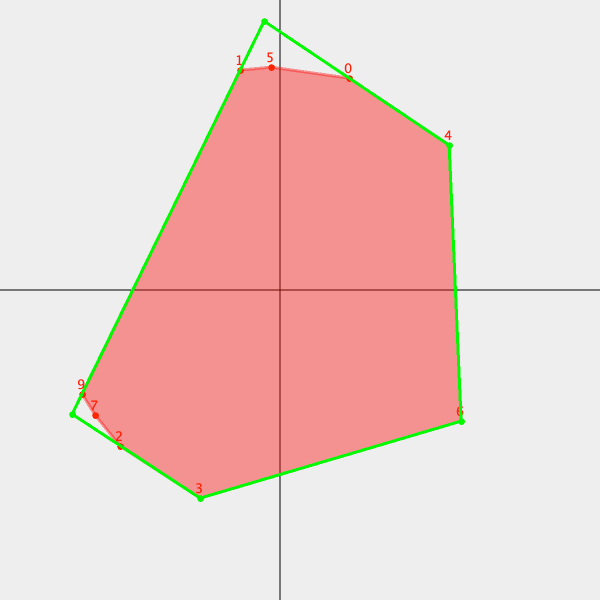
\includegraphics[width=0.3\textwidth]{media/LessArea/9_5.png} \\
        (a) E = 5, h = 4 & (b) E = 7, h = 5 & (c) E = 9, h = 5
    \end{tabular}
\end{figure}

I poligoni prodotti da questo algoritmo tendono a rappresentare in modo accurato 
la forma originale del poligono. 
Tuttavia, l'algoritmo presenta due criticità: la selezione dei lati diventa più 
complessa con l'aumentare del numero di lati del poliedro, poiché in media sarà necessario 
calcolare proiezioni pari alla metà dei lati, e la scelta degli iperpiani non garantisce 
necessariamente la generazione di un politopo chiuso.
 
\pagebreak
\subsection{Ipotesi di Algoritmo Cutting Edges}

Questo algoritmo prevede la graduale selezione degli iperpiani ideali. Questa avviene tramite 
il calcolo delle aree eccedenti per ciascun lato: i lati con le aree eccedenti 
minori saranno scelti per essere approssimati tramite il prolungamento dei lati a loro adiacenti. 

\begin{figure}[H]
    \centering
    \begin{tabular}{c}
        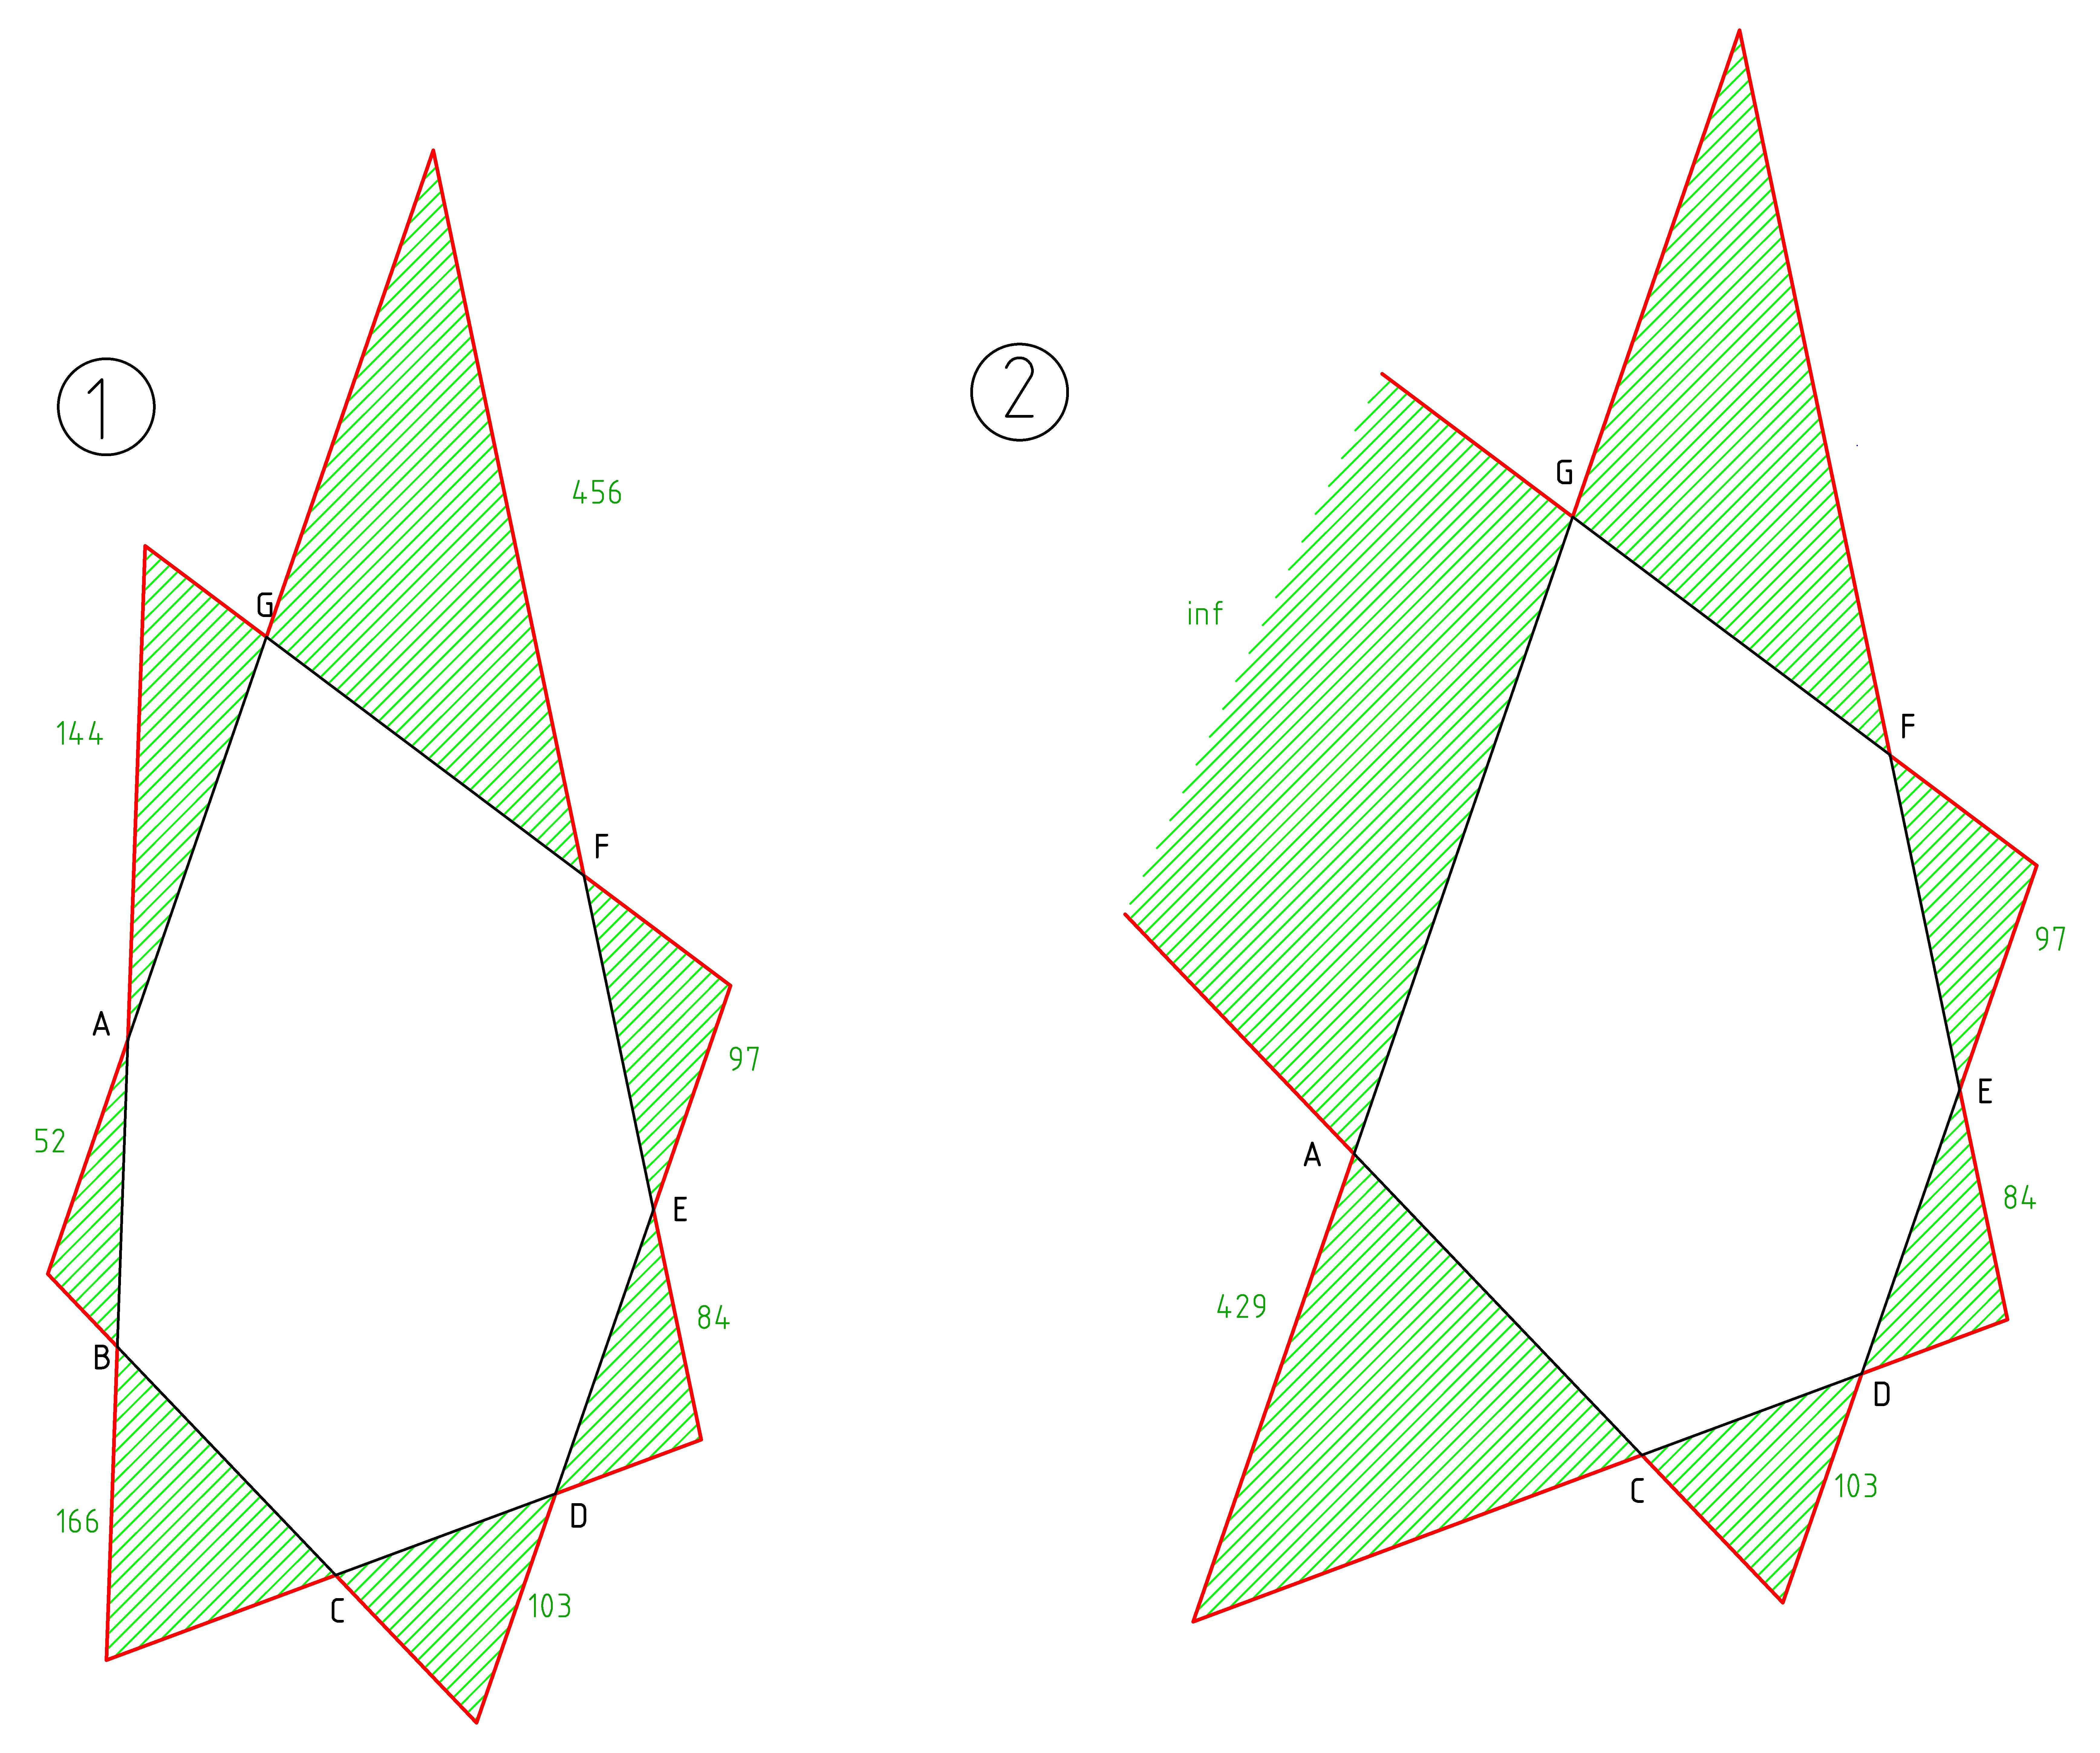
\includegraphics[width=0.8\textwidth]{media/Demo_algorithms/demo_cutting_edges.jpg} \\
        \begin{tabular}{l}
            (1) Dimostrazione del criterio di scelta dell'iperpiano migliore secondo C.E.\\
            (2) Dimostrazione del criterio di scelta sul restante politopo
        \end{tabular}
    \end{tabular}
\end{figure}

\begin{center}
    Esempi di approssimazione:
\end{center}
\begin{figure}[H]
    \centering
    \begin{tabular}{ccc}
        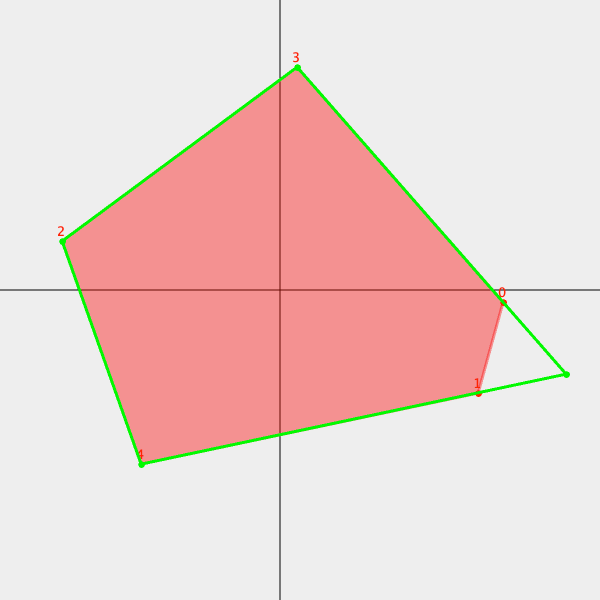
\includegraphics[width=0.3\textwidth]{media/LessArea/5_4.png} &
        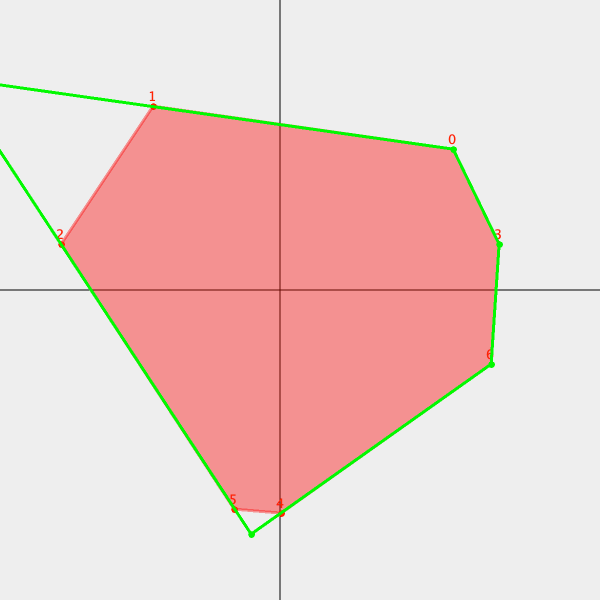
\includegraphics[width=0.3\textwidth]{media/LessArea/7_5.png} &
        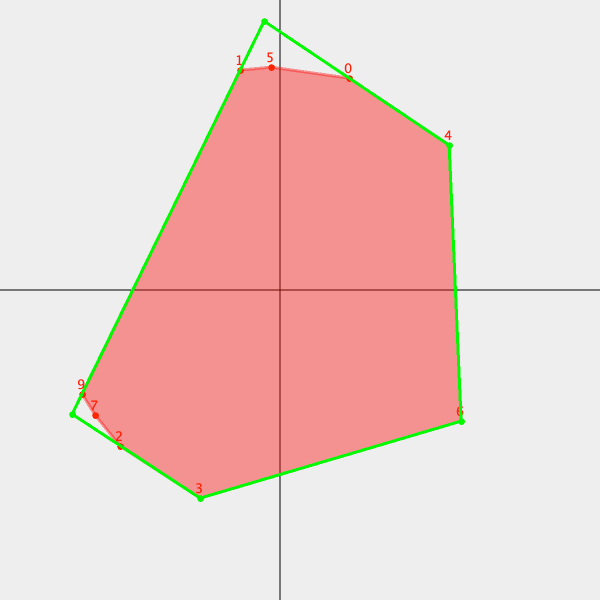
\includegraphics[width=0.3\textwidth]{media/LessArea/9_5.png} \\
        (a) E = 5, h = 4 & (b) E = 7, h = 5 & (c) E = 9, h = 5
    \end{tabular}
\end{figure}

I poligoni generati sembrano rappresentare fedelmente la forma originale del guscio 
convesso e, allo stesso tempo, questi rispettano il vincolo di contenere tutti i punti 
ammissibili del poliedro originale.
L'algoritmo può inoltre trarre vantaggio dall'utilizzo di una mappa per poter 
evitare il ripetuto calcolo delle aree non modificate dall'approssimazione.
\\


\chapter{Analisi delle sperimentazioni}
\section{Tipo di testing}
Per la fase di testing sono stati selezionati gli algoritmi che sono in grado di rispettare
almeno la seconda delle condizioni poste in principio, risultano perciò esclusi CLA e CSA.\\

Il testing è stato condotto con codice Java tramite la generazione di poligoni convessi
randomici con un numero sempre crescenti di lati $E$ (4 - 30). 
Per ogni $E$ vengono creati 5 politopi differenti e, per ognuno di questi, verranno creati
$E-3$ casi di test, ciascuno con un budget di iperpiani crescente $3 .. E$
per un numero totale di 1729 casi di test sottoposti a ciascun algoritmo.

L'algoritmo utilizzato per la generazione randomica dei poliedri convessi 
è l'algoritmo di Valt, spiegato estensivamente nel rispettivo documento
\cite{ValtrAlgorithm}.

\subsection*{Metriche di valutazione}
Oltre al tempo di esecuzione dei vari algoritmi, per valutarne l'accuratezza si è deciso
di utilizzare l'indice di Jaccard, ampiamente impiegato nella teoria degli insiemi. 
Questo indice misura la somiglianza tra due insiemi calcolando il rapporto tra 
l'intersezione e l'unione degli stessi, ovvero:
 
\[
J(A, B) = \frac{|A \cap B|}{|A \cup B|}
\]

Applicando tale principio ai politopi, si può valutare il rapporto tra il politopo originale 
e quello approssimato. In particolare, l'indice di Jaccard consente di stimare il volume 
eccedente rispetto al volume del politopo originale con valori compresi tra 0 e 1.\\

Dopo aver eseguito il test, i risultati vengono immagazzinati in una tabella csv per poter 
effettuare delle analisi tramite l'utilizzo di librerie Python.


\subsection*{Limiti del testing}
Un limite fondamentale dell'algoritmo di generazione di gusci convessi in due dimensioni 
consiste nel fatto che, all'aumentare del numero di lati del poiliedro generato, 
la forma che questo assumerà sarà sempre più probabilmente simile ad una forma
ben stabilita in questa ricerca di Pavel Valt.\cite{probabilityConvexhull2d}

\pagebreak
\section{Analisi dei dati} 
\label{sec:Analisi dei dati}
I risultati ottenuti evidenziano che gli algoritmi che selezionano gli iperpiani 
per creare l'approssimazione possono generare politopi aperti. In particolare, 
l'algoritmo \textit{LessArea} è quello più incline a produrre politopi di approssimazione aperti, 
fenomeno osservato in 23 casi su un totale di 1729.\\
Anche l'algoritmo \textit{BoxCutting} può occasionalmente generare politopi aperti, 
sebbene questo accada con minore frequenza. 
Grazie alla sua euristica evolutiva nella selezione degli iperpiani, 
sono stati riscontrati solo 7 casi su 1729. Questo comportamento si manifesta principalmente 
in presenza di politopi iniziali con un elevato numero di facce e con budget di iperpiani 
molto limitato.

Le probabilità complessive che si verifichi questo evento risultano tuttavia 
non influenti al fine dell'analisi sulle statistiche ($\leq 1\%$).

Come evidenziato nella tabella \ref{tab:results} i dati risultano essere nettamente a favore di
alcuni algoritmi che riescono ad ottenere dei buoni risultati apportando allo stesso
tempo tempi di esecuzione in media inferiori.

\begin{table}[h] 
    \centering
    \begin{tabular}{|c|c|c|}
        \hline
        Algoritmo & Jaccard Index & Tempo Medio (Millisec) \\
        \hline
        BoxCutting              & 0.90  & 1.67\\
        CuttingEdges            & 0.94  & 0.59\\ 
        CuttingLargerAngle2     & 0.91  & 0.70 \\
        CuttingSmallerAngle2    & 0.48  & 0.69 \\
        DistanceFromG           & 0.69  & 4.00 \\
        LessArea                & 0.74  & 298.76 \\
        \hline
    \end{tabular}
    \caption{Tabella riassuntiva delle prestazioni delle euristiche} 
    \label{tab:results}
\end{table} 

Dato l'elevato costo computazionale dell'euristica LessArea, i seguenti grafici
non conterranno le informazioni inerenti a questo Algoritmo.

\subsection*{Tempi di esecuzione}

\begin{figure}[H]
    \centering
    \begin{minipage}[b]{0.45\textwidth}
        \centering
        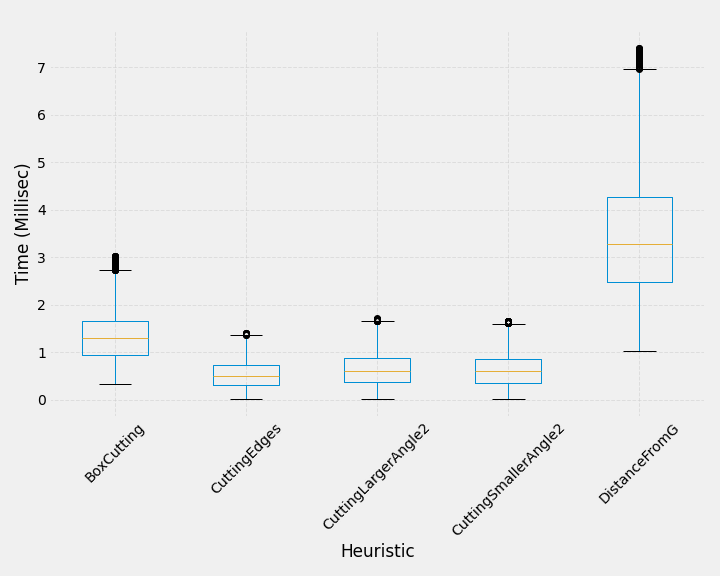
\includegraphics[width=\textwidth]{media/report/bxplt_time.png}
        \caption{boxplot del tempo medio di esecuzione per ciascuna euristica.\\
        }
    \end{minipage}
    \hspace{0.05\textwidth}
    \begin{minipage}[b]{0.45\textwidth}
        \centering
        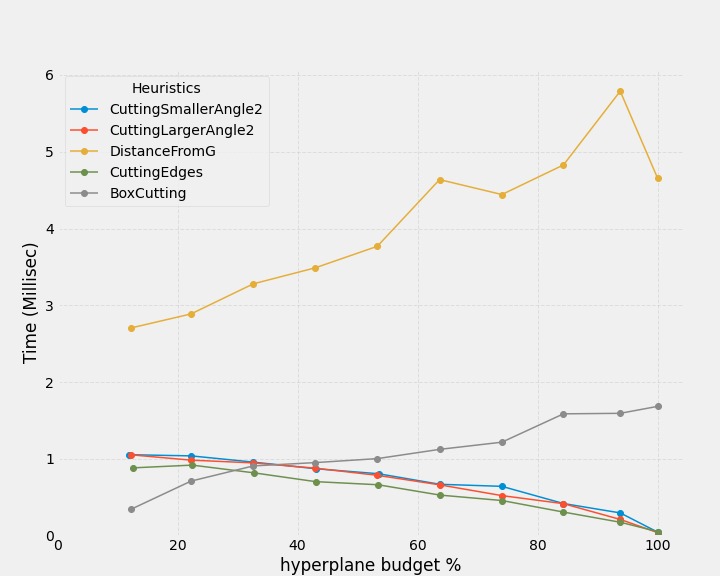
\includegraphics[width=\textwidth]{media/report/Time_plot.png}
        \caption{andamento dei tempi di esecuzione di ciascuna euristica in base al budget di iperpiani $h$.}
        \label{fig: time_h}
    \end{minipage}
\end{figure}

Osservando i tempi medi di esecuzione degli algoritmi si possono discernere due principali
classi di algoritmi, il primo dei quali ha un tempo di esecuzione nettamente inferiore rispetto al secondo.
In particolare dal grafico in Figura \ref*{fig: time_h} si distinguono fra tutti gli algoritmi BoxCutting e CuttingEdge 
che risultano essere più efficienti per differenti budget di iperpiani.

\subsection*{Accuratezza}

\begin{figure}[H]
    \centering
    \begin{minipage}[b]{0.45\textwidth}
        \centering
        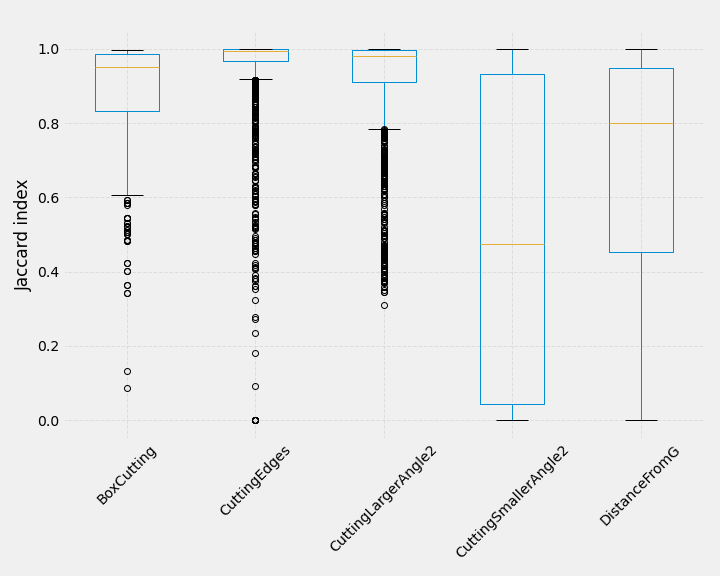
\includegraphics[width=\textwidth]{media/report/bxplt_jaccard.png}
        \caption{boxplot dell'accuratezza del politopo di approssimazione per ciascuna euristica.}
    \end{minipage}
    \hspace{0.05\textwidth}  
    \begin{minipage}[b]{0.45\textwidth}
        \centering
        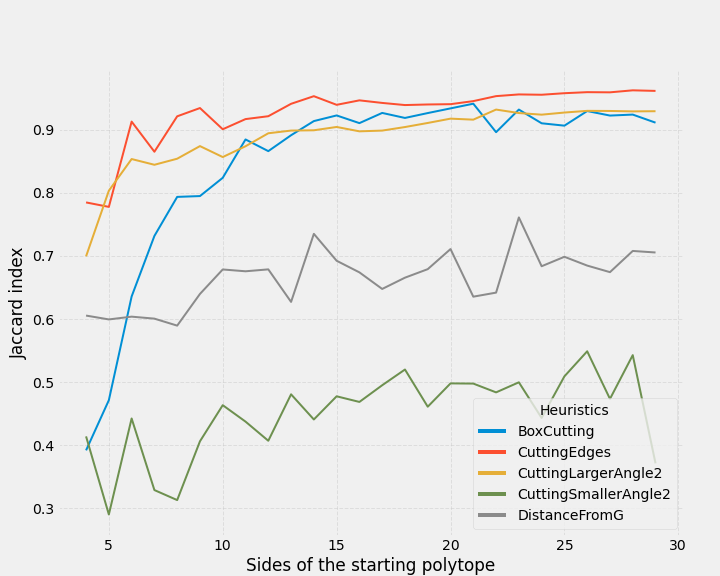
\includegraphics[width=\textwidth]{media/report/Accuracy_plot.png}
        \caption{andamento dell'accuratezza di approssimazione di ciascuna euristica in base al numero di lati del poligono iniziale.}
    \end{minipage}
\end{figure}

I due grafici sovrastanti espongono con quale costanza e quale accuratezza i politopi 
di approssimazione generati dagli algoritmi rappresentino il politopo di partenza.\\
Si può notare inoltre come un gruppo di algoritmi riesca a mantenere una
precisione costantemente piu accurata rispetto ad altri.

\chapter{Elevazione a n-dimensioni}

\section{Passi logici}
Date le conclusioni precedenti, si è deciso di procedere con lo sviluppo n-dimensionale
delgi algoritmi CuttingEdge e BoxCutting.
Poiché entrambi prevedono il calcolo delle aree, in più dimensioni richiederanno il 
calcolo di volumi n-dimensionali. 
Questi, come è noto, con l'aumentare delle dimensioni, avranno un grado di complessità
di calcolo sempre maggiore. Sono perciò previsti tempi di esecuzione gradualmente maggiori.

L'elevazione dell'algoritmo da semplice codice Java richiede l'utilizzo di strumenti 
avanzati, come Polymake, che consente di manipolare i poliedri con maggiore facilità, 
e del linguaggio Perl, con cui il software Polymake mostra una forte integrazione.

\subsection{L'algoritmo CuttingEdge n-dimensionale}
L'algoritmo CuttingEdge viene applicato a un poliedro di dimensione arbitraria 
con un budget prestabilito di iperpiani disponibili $h$. 
Il politopo iniziale utilizzato per l'approssimazione coincide con il poliedro originale.

Il processo per ogni faccia del poliedro si articola nei seguenti passi:

\begin{enumerate} 
    
    \item Individuazione dei coefficienti della faccia.
    
    \item Costruzione del politopo dato dal prolungamento degli iperpiani adiacenti
    a questa (inversione dei coefficienti della faccia);

    \item Individuazione del volume del politopo costruito;
    
    \item Selezione del'iperpiano producente il politopo con il volume inferiore fra
    tutti;

\end{enumerate}

Una volta individuato l'iperpiano migliore, questo viene rimosso dal politopo di approssimazione.

\subsection{L'algoritmo BoxCutting n-dimensionale}
Dato un poliedro in una dimensione arbitraria e $h$ rappresentante
il budget di iperpiani disponibili, 
viene costruito il parallelepipedo (Bounding Box) n dimensionale che lo racchiude.\\

L'algoritmo poi per ciascuna faccia procede come segue:

\begin{enumerate}
    
    \item Individuazione dei coefficienti della faccia;

    \item Costruzione del politopo incluso fra la faccia e la Bounding Box;
    
    \item Calcolo del volume del suddetto politopo;

    \item Selezione dell'iperpiano con il rispettivo volume maggiore;

\end{enumerate}

Una volta determinato l'iperpiano scelto, viene rimosso dalla bounding box il corrispettivo
volume compreso. L'insieme di iperpiani scelti determinerà il poliedro di approssimazione.

\section{Il Codice}
Per il calcolo del volume di un poliedro n-dimensionale esistono differenti metodi illustrati 
in questo documento: \cite{nDvolume} in cui è stata trovata una formula specifica.

Grazie all'utilizzo del software Polymake molte delle operazioni computazionalmente
rilevanti, come l'inversione dei semispazi o la rimozione/aggiunta di 
iperpiani ad un politopo, possono essere facilmente integrate nel codice.\\
Per la futura analisi è di importanza rilevante anche considerare che l'algoritmo 
CuttingEdge è stato dotato di una mappa per risparmiare operazioni di 
calcolo dei volumi ripetitive.

\subsection*{I politopi creati}

Esempio visivo in diverse angolazioni di uno step di approssimazione di un poliedro 
in 3 dimensioni.

\begin{figure}[H]
    \centering
    
    \newcounter{immagine} % Definizione del contatore
    \forloop{immagine}{1}{\value{immagine} < 5}{%
        \includegraphics[width=0.2\textwidth]{media/3Dproof/CuttingEdge/immagine\theimmagine.png} % Uso di \theimmagine per il numero del contatore
    }
    
    \caption{Esempio di approssimazione iniziale dell'algoritmo CuttingEdge}
\end{figure}

\begin{figure}[H]
    \centering
    
    \newcounter{img} % Definizione del contatore
    \forloop{img}{1}{\value{img} < 5}{%
        \includegraphics[width=0.2\textwidth]{media/3Dproof/BoxCutting/immagine\theimg.png} % Uso di \theimmagine per il numero del contatore
    }
    
    \caption{Esempio di approssimazione iniziale dell'algoritmo BoxCutting}
\end{figure}

\chapter{Analisi a n-dimensioni}
\section{Tipo di testing}

Il testing eseguito si basa interamente sul software Polymake.
Sulla falsa linea di quello che è stato fatto in precedenza si sono generati dei casi di test:
per ogni dimensione sono stati generati 5 politopi randomici, ciascuno con un numero definito 
di iperpiani che va da $dim+2$ a $dim+7$.
Per evitare di interrogare l'algoritmo con un budget di iperpiani ogni volta 
decrescente, si è provveduto a interrogare una unica volta l'algoritmo fornendo il politopo
da approssimare, per ogni approssimazione eseguita vengono registrati i 
rispettivi dati dell'esecuzione.\\


\section{Analisi dei dati}

\begin{figure}[H]
    \centering
        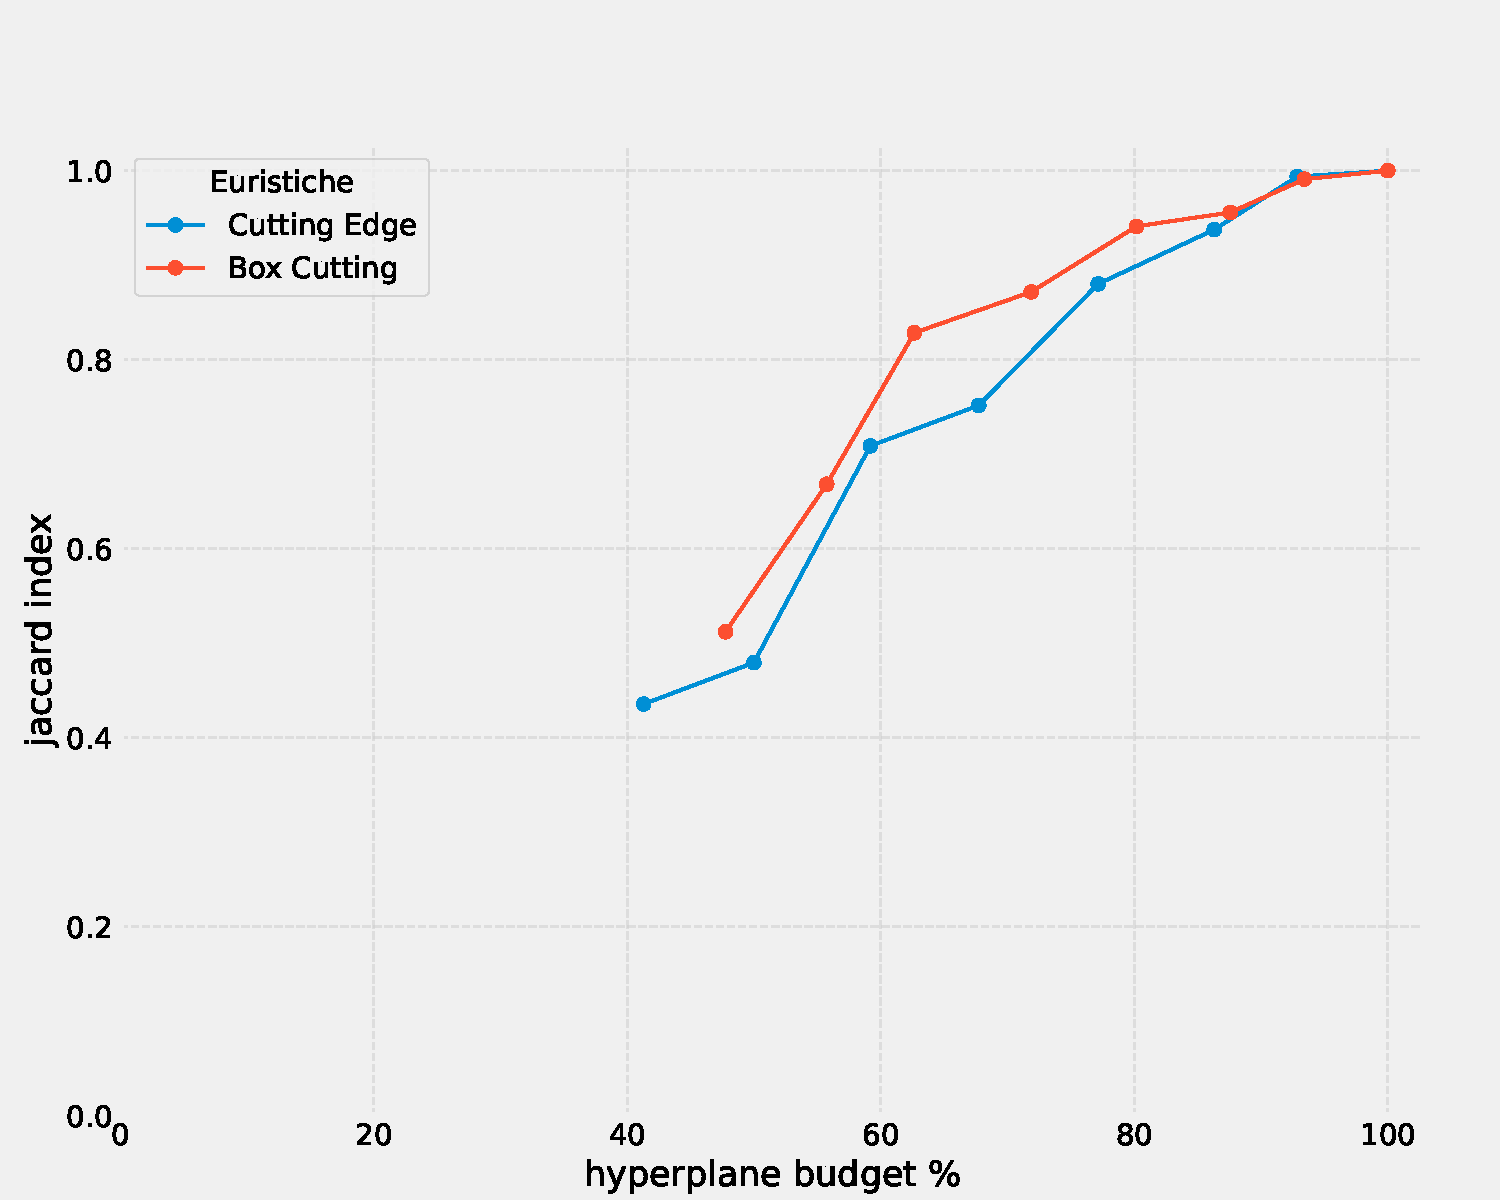
\includegraphics[width=0.7\textwidth]{media/report_ndim/ndim_jaccard.pdf} \\
        \caption{Andamento dell'accuratezza delle approssimazione degli algoritmi 
        al crescere del budget di iperpiani a disposizione}
\end{figure}

\begin{figure}[H]
    \centering
    \begin{minipage}[b]{0.45\textwidth}
        \centering
        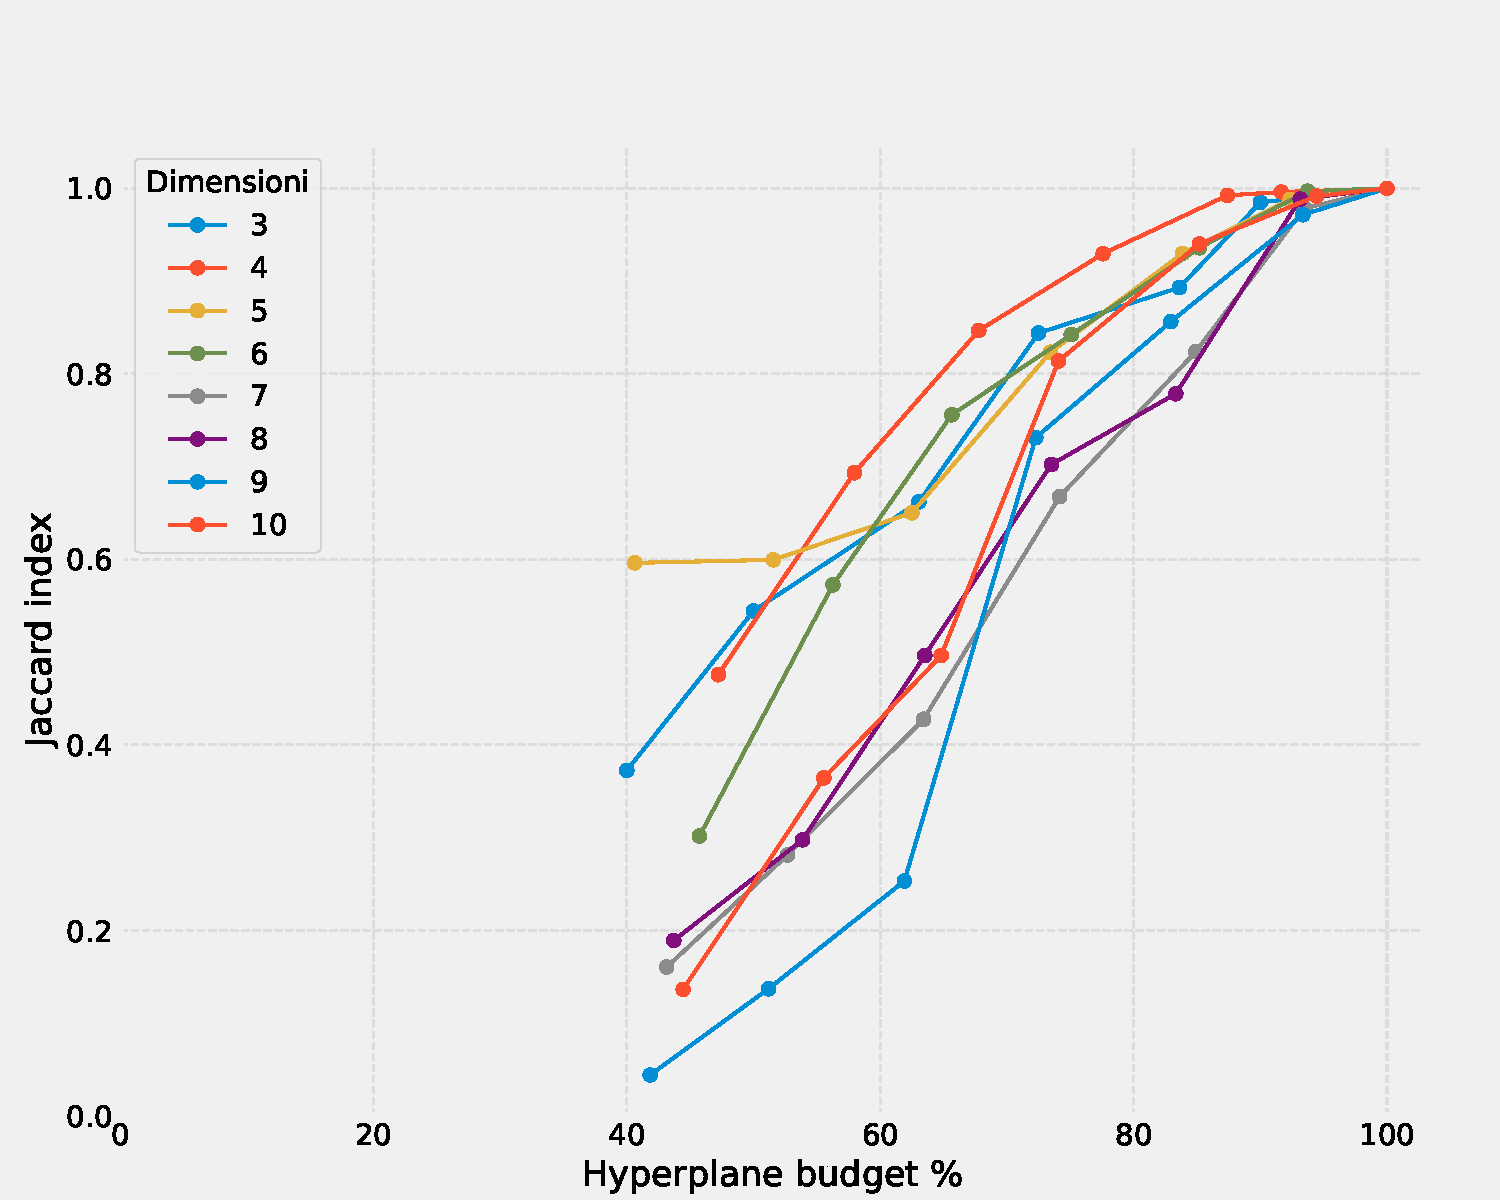
\includegraphics[width=\textwidth]{media/report_ndim/ndim_accuracy_diff_CE.pdf}
        \caption{Accuratezza dell'approssimazione di CuttingEdge al crescere di h.}
        \label{fig: acc_ce}
    \end{minipage}
    \hspace{0.05\textwidth}  % Spazio orizzontale tra le immagini
    \begin{minipage}[b]{0.45\textwidth}
        \centering
        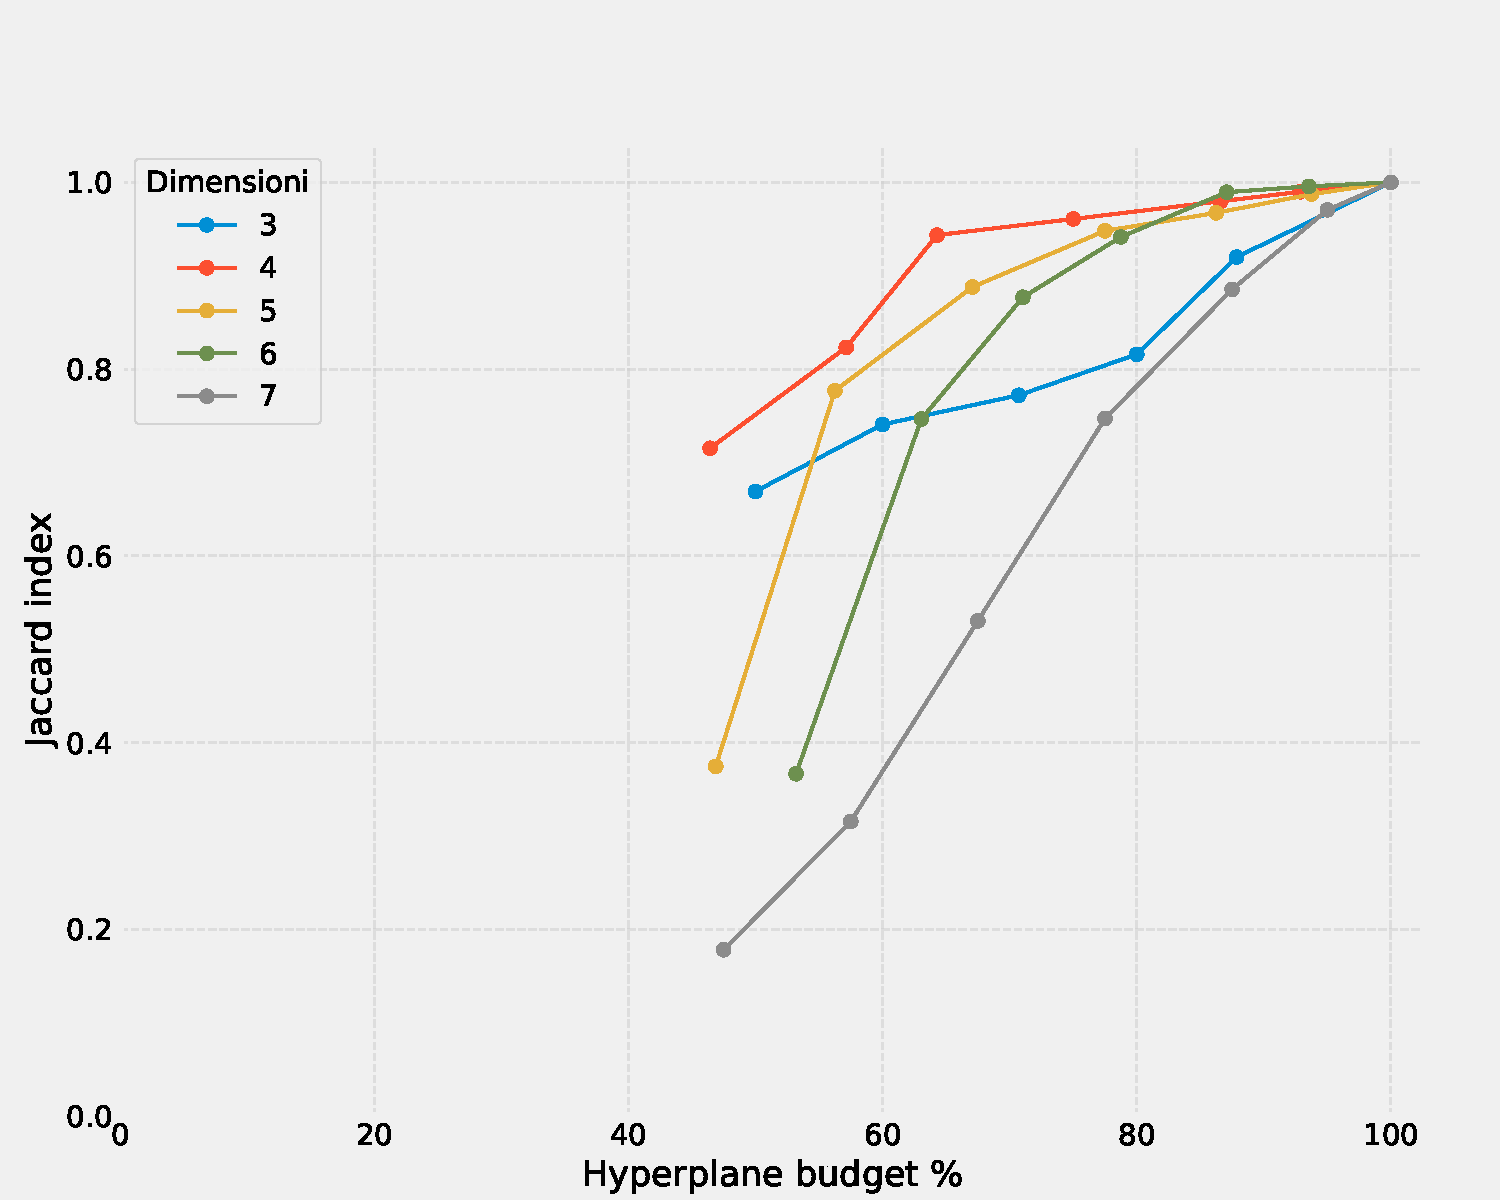
\includegraphics[width=\textwidth]{media/report_ndim/ndim_accuracy_diff_BC.pdf}
        \caption{Accuratezza dell'approssimazione di BoxCutting al crescere di h.}
        \label{fig: acc_bc}
    \end{minipage}
\end{figure}
Come previsto, il budget di iperpiani per l'approssimazione è incisivo sulla precisione
degli algoritmi. Nonostante ciò, è doveroso notare che entrambi gli algoritmi sembrano
avere un comportamento analogo al variare del budget di iperpiani.\\

Analizzando nello specifico il comportamento degli algritmi al variare delle dimensioni,
(Figure \ref*{fig: acc_ce} e \ref*{fig: acc_bc}) si nota un comportamento pressochè 
invariato per CuttingEdge mentre per BoxCutting il numero di dimensioni 
sembra marginalmente influenzare influenzarne l'accuratezza delle approssimazioni.

\begin{figure}[H]
    \centering
    \begin{tabular}{c}
        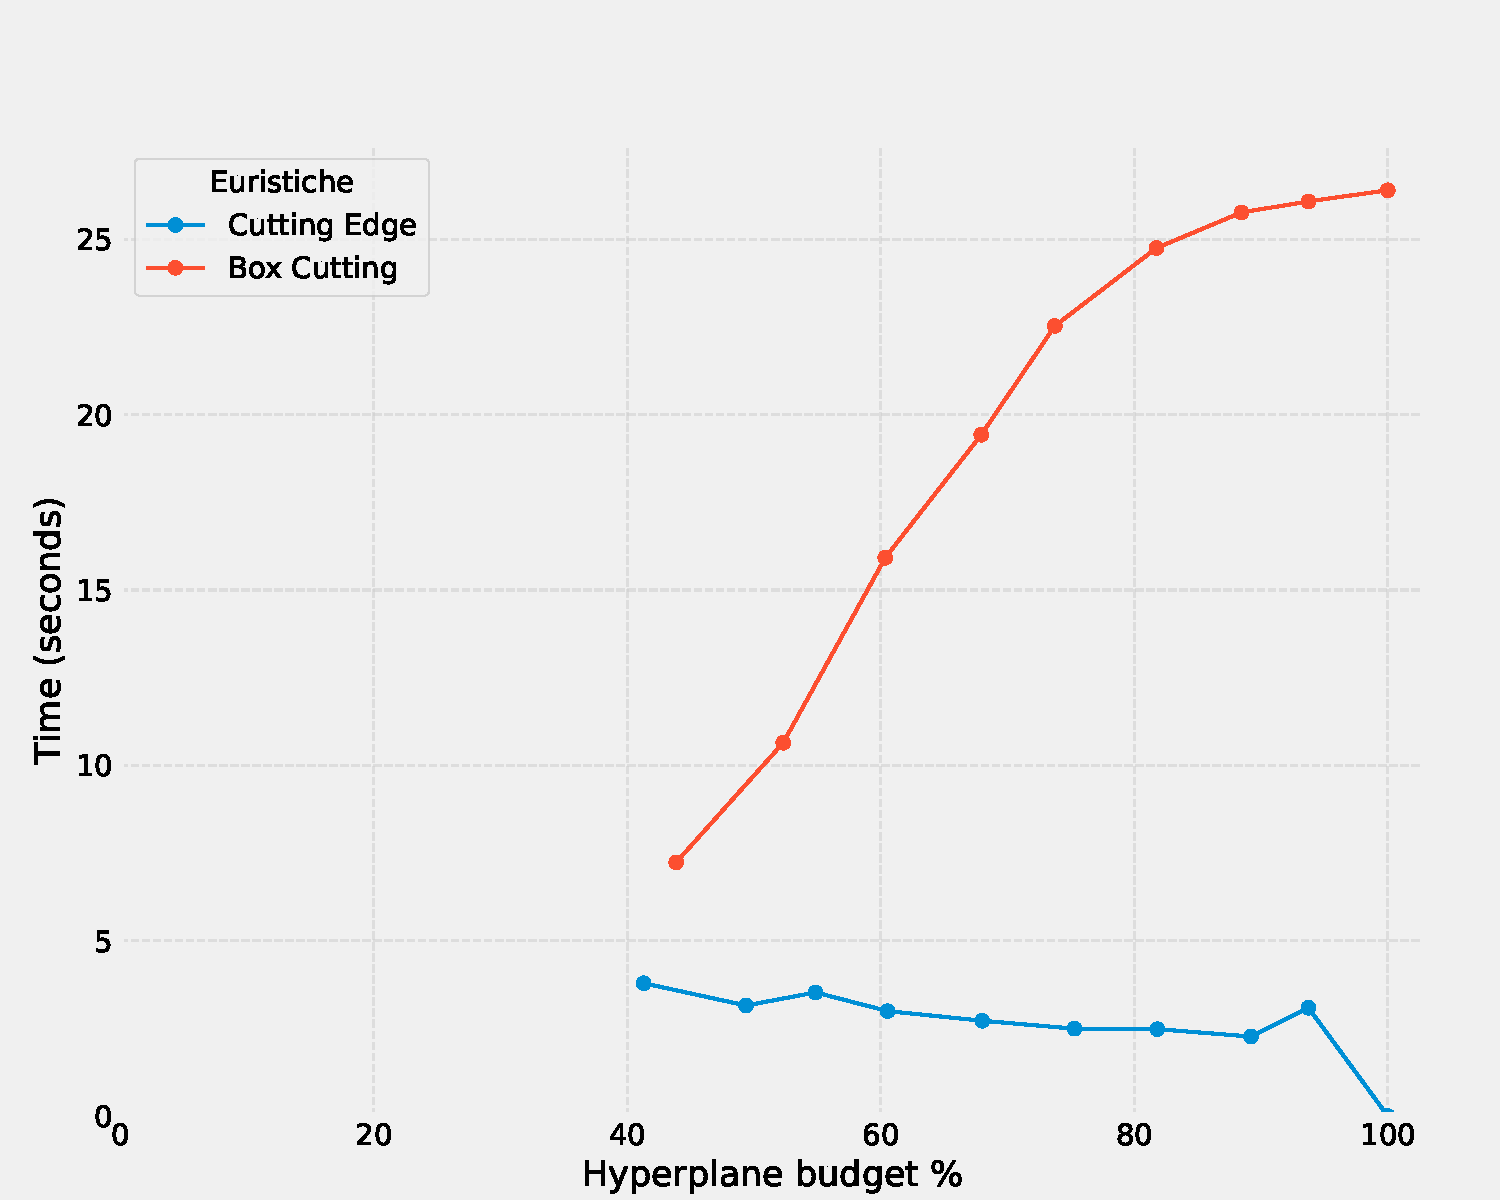
\includegraphics[width=0.7\textwidth]{media/report_ndim/ndim_time.pdf} \\
    \end{tabular}
    \caption{Grafico dei tempi di calcolo medi al variare del budget di iperpiani 
    a diposizione degli algoritmi scelti}
\end{figure}

Confrontando i tempi di calcolo si può notare una notevole differenza fra i due dovuta
principalmente dalla campacità di memorizzazione dei volumi calcolati per l'algoritmo 
CuttingEdge.


\begin{figure}[H] 
    \centering
    \begin{minipage}[b]{0.45\textwidth}
        \centering
        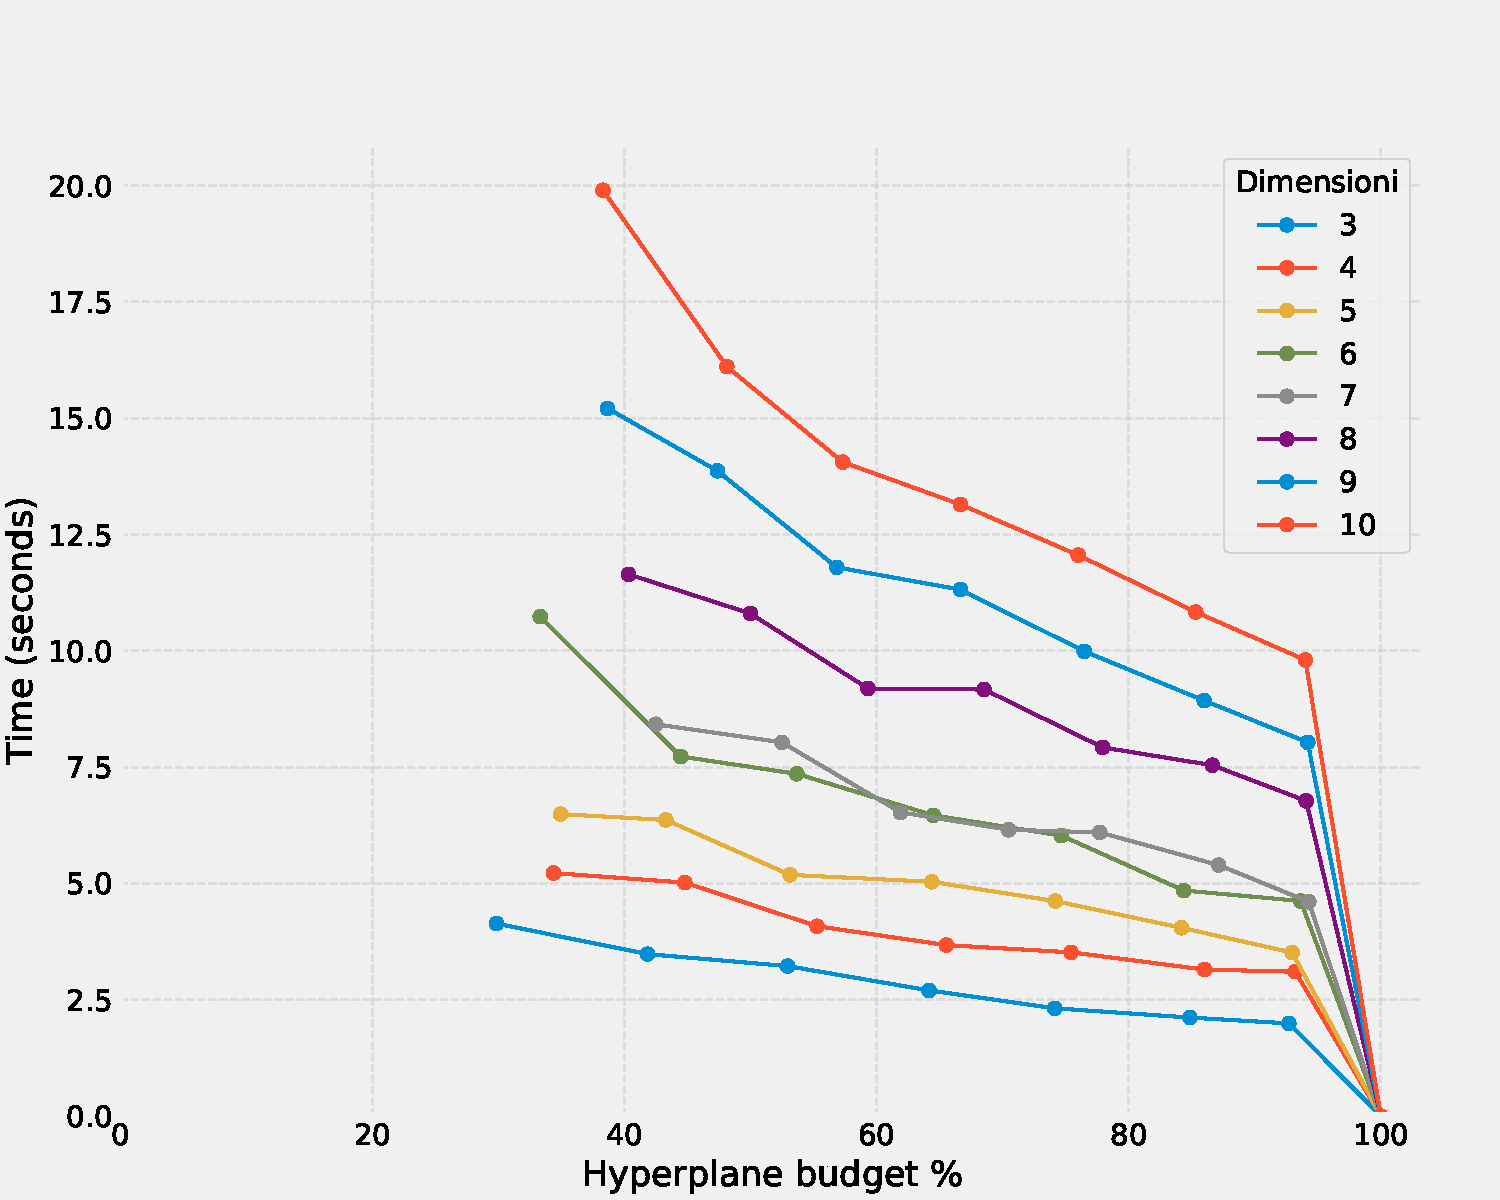
\includegraphics[width=\textwidth]{media/report_ndim/ndim_time_diff_CE.pdf}
        \caption{Tempi di esecuzione dell'euristica CuttingEdge al variare del 
        budget di iperpiani.}
        \label{fig: disp_ce}
    \end{minipage}
    \hspace{0.05\textwidth}  % Spazio orizzontale tra le immagini
    \begin{minipage}[b]{0.45\textwidth}
        \centering
        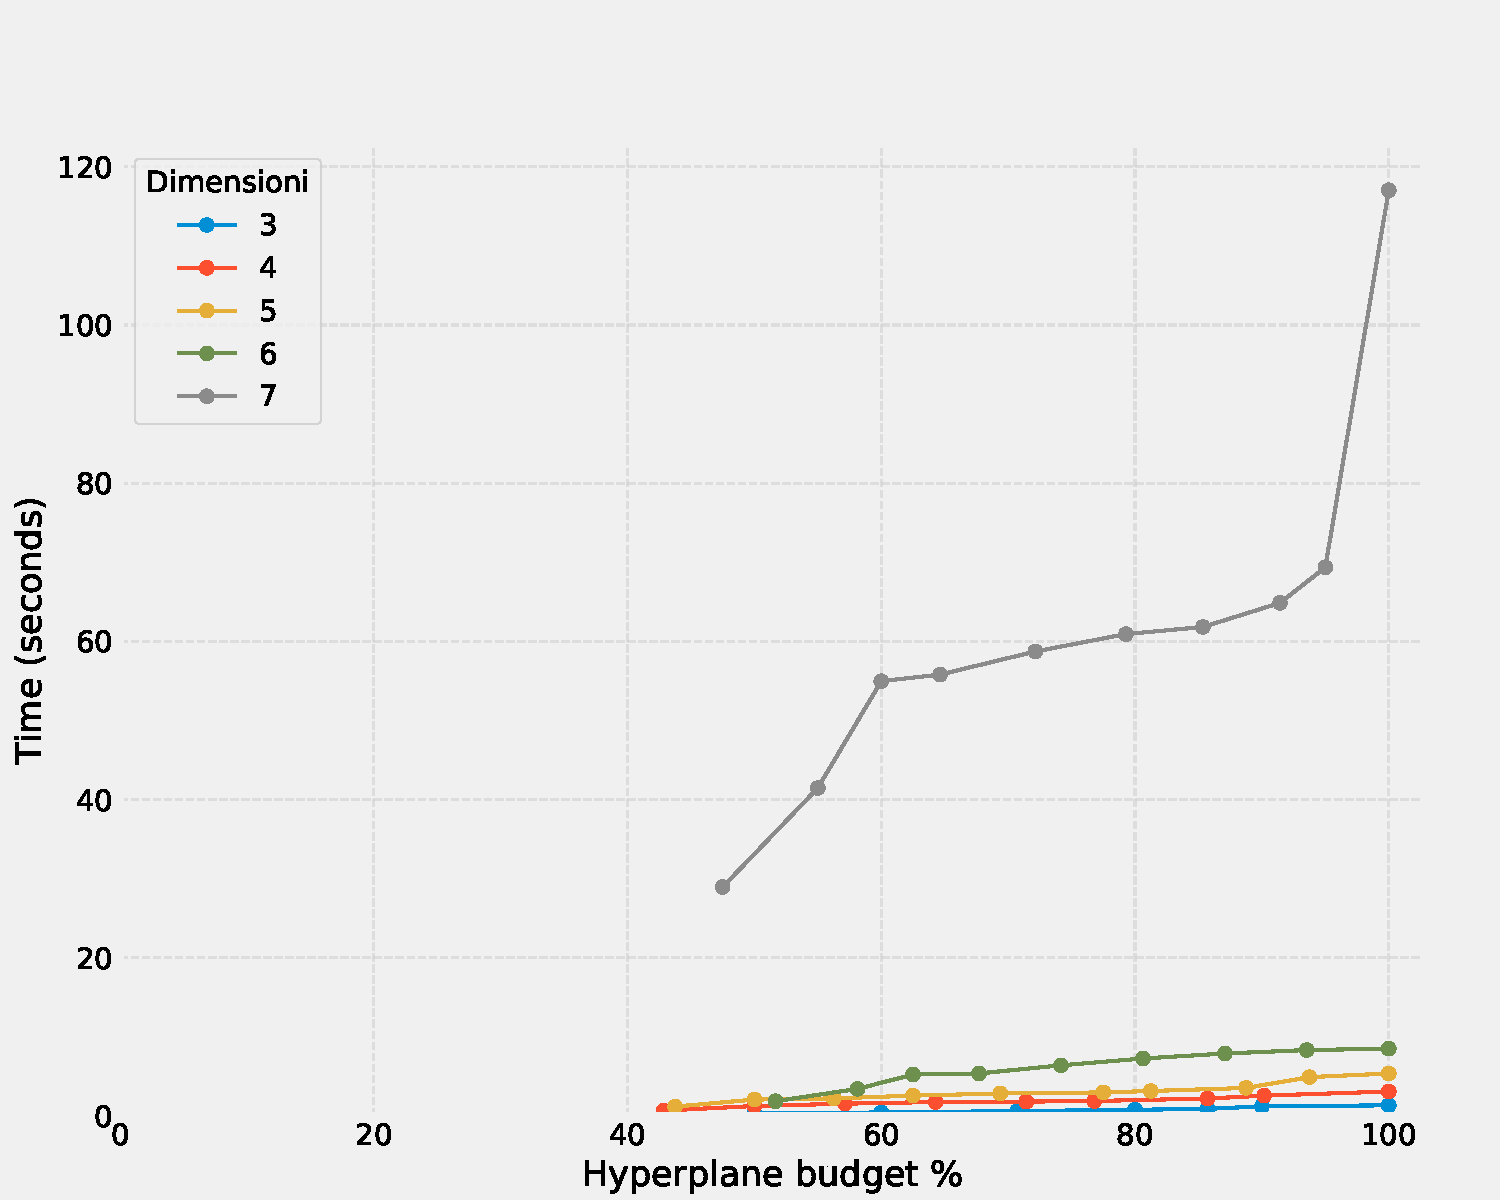
\includegraphics[width=\textwidth]{media/report_ndim/ndim_time_diff_BC.pdf}
        \caption{Tempi di esecuzione dell'euristica BoxCutting al variare 
        del budget di iperpiani.}
        \label{fig: disp_bc}
    \end{minipage}
\end{figure}

\begin{figure}[H]
    \centering
    \begin{minipage}[b]{0.45\textwidth}
        \centering
        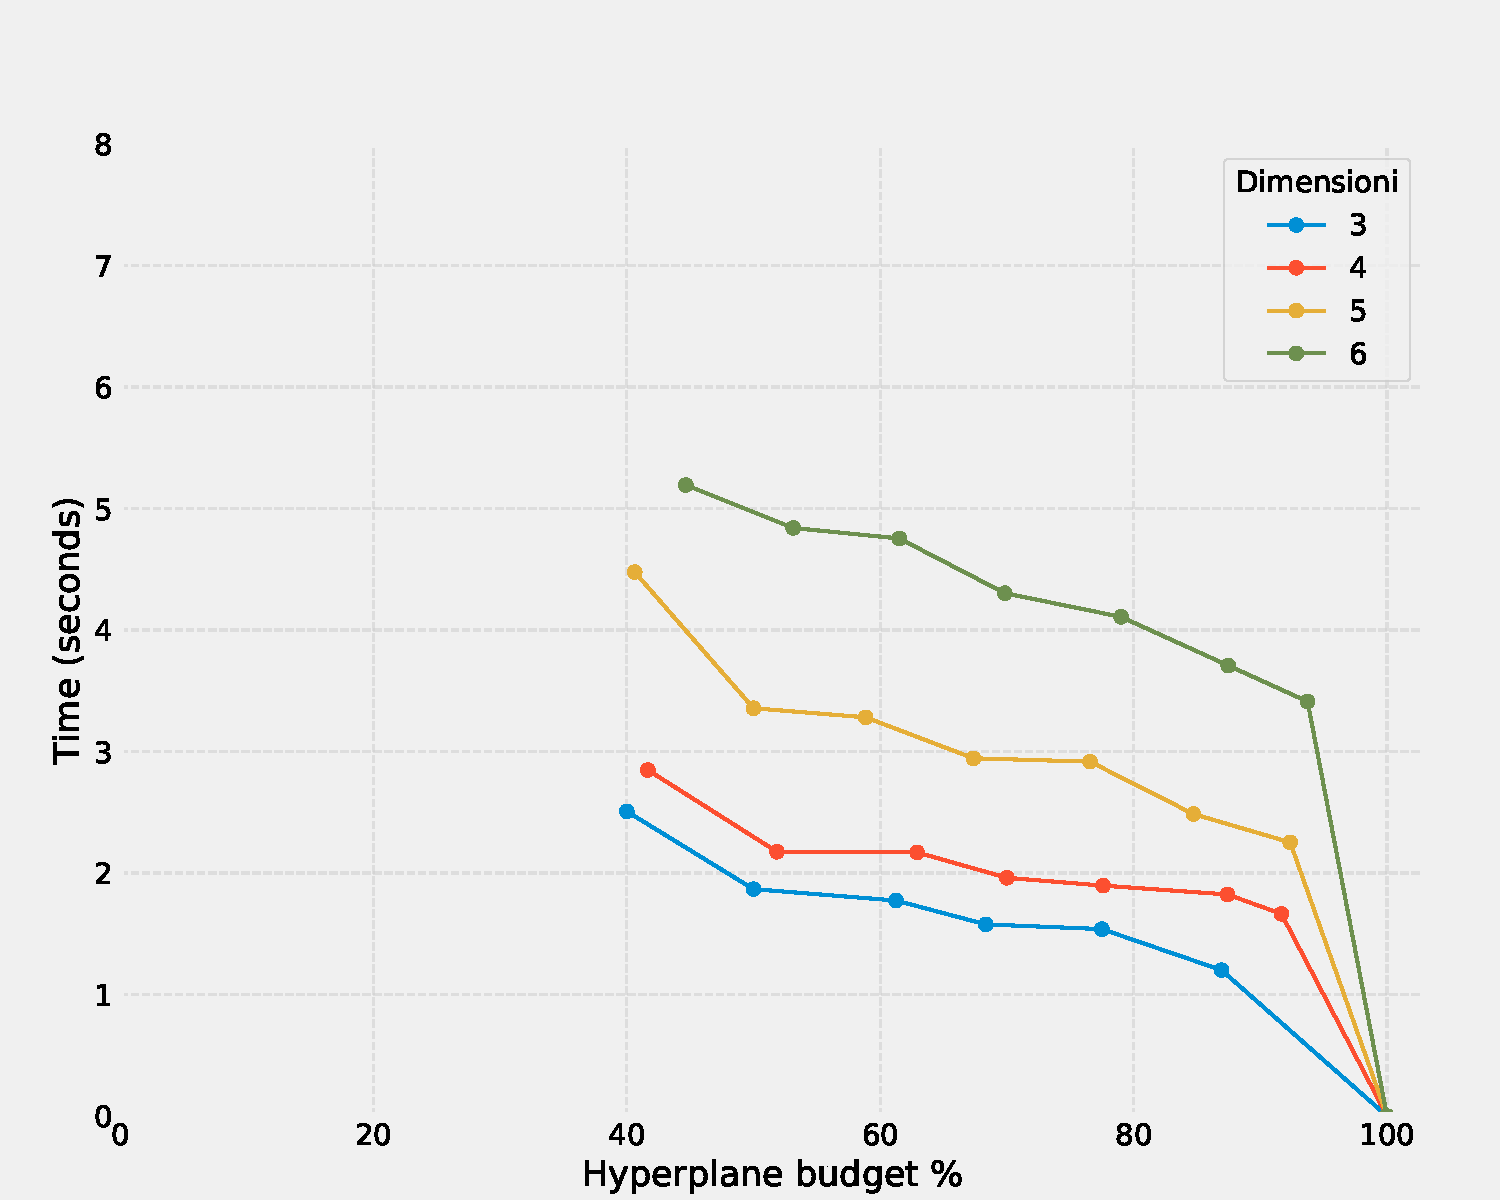
\includegraphics[width=\textwidth]{media/report_ndim/ndim_time_diff_CE_under7.pdf}
        \caption{Tempi di esecuzione dell'euristica CuttingEdge al variare 
        del budget di iperpiani per le dimensioni comprese tra 3 e 6, 
        filtrando le dimensioni superiori per una migliore visualizzazione.}
        \label{fig: disp_ce_sub7}
    \end{minipage}
    \hspace{0.05\textwidth}  % Spazio orizzontale tra le immagini
    \begin{minipage}[b]{0.45\textwidth}
        \centering
        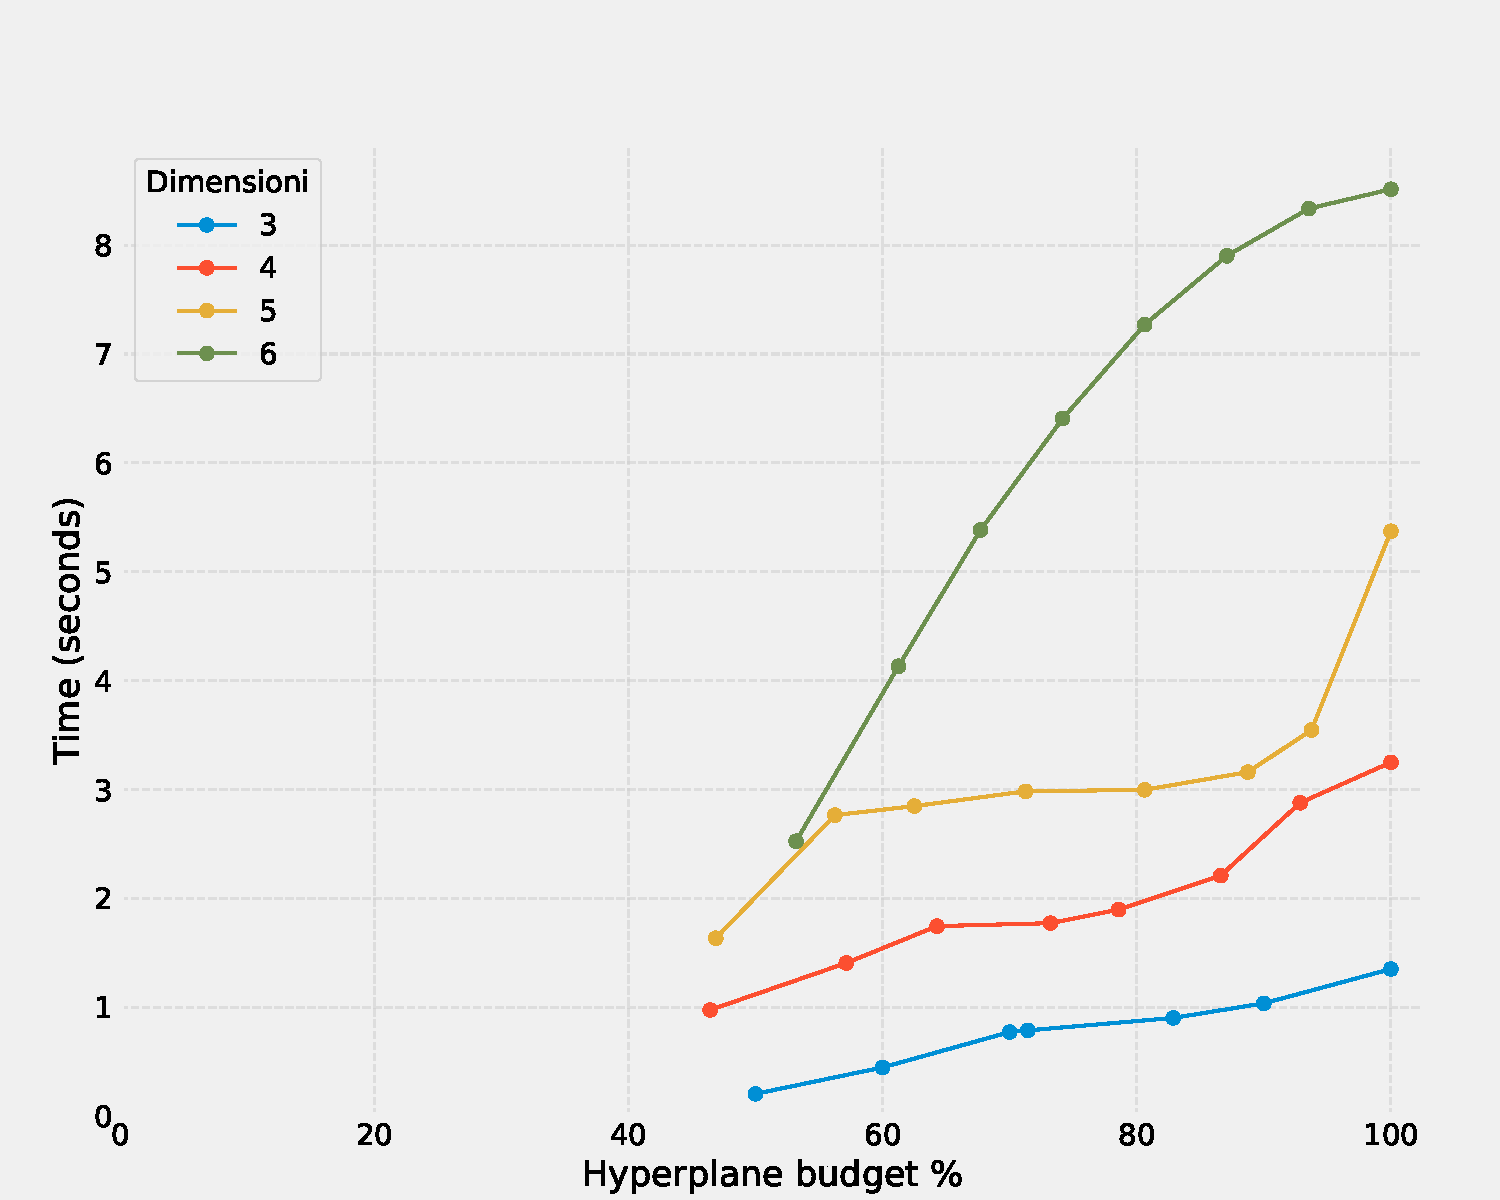
\includegraphics[width=\textwidth]{media/report_ndim/ndim_time_diff_BC_under7.pdf}
        \caption{Tempi di esecuzione dell'euristica BoxCutting per lo stesso 
        intervallo di dimensioni.\\
        \\}
        \label{fig: disp_bc_sub7}
    \end{minipage}
\end{figure}

Come si può evincere dai grafici nelle Figure \ref{fig: disp_ce} \ref{fig: disp_bc},
al crescere delle dimensioni dei politopi di partenza l'euristica BoxCutting 
subisce una notevole crescità del tempo computazionale, mentre CuttingEdge 
riesce a mantenere una crescita costante e predicibile.

Confrontando le dimensioni per le quali i due algoritmi risultano comparabili, 
ovvero dalla 3 alla 6 (Figure \ref{fig: disp_ce_sub7} \ref{fig: disp_bc_sub7}), 
si può osservare che entrambi gli algoritmi 
presentano tempi di esecuzione simili, ma con andamenti di crescita opposti. 
In particolare, l'algoritmo CuttingEdge mostra un tempo di esecuzione decrescente 
all'aumentare del budget di iperpiani, mentre l'algoritmo BoxCutting evidenzia 
una crescita dei tempi con l'incremento del budget di iperpiani. 
Questa caratteristica può renderli adatti per scopi differenti.\\



\chapter{Conclusioni}

\section{Sintesi dei risultati ottenuti}
Tra gli algoritmi analizzati, i due che hanno mostrato i risultati più promettenti 
sono CuttingEdge e BoxCutting, i quali adottano approcci opposti per la risoluzione del problema. 
CuttingEdge parte dal poliedro completo e, ad ogni passo, riduce il numero di 
iperpiani che definiscono la sua approssimazione. BoxCutting, al contrario, 
inizia da una forma approssimata con il numero minimo di lati e aggiunge gradualmente 
nuovi iperpiani fino a ricostruire il poliedro originale.\\

Nonostante CuttingEdge si sia dimostrato superiore in termini di prestazioni, 
e di stabilità al variare delle dimensioni dei politopi 
grazie al ridotto numero di calcoli dei volumi, entrambi gli algoritmi 
risultano particolarmente adatti a scenari specifici:
BoxCutting per casi in cui si desidera ottenere un'approssimazione con 
un numero molto ridotto di iperpiani, oppure per la creazione di approssimazioni con poliedri aperti,
mentre CuttingEdge si presta meglio in casi in cui è necessaria un'approssimazione con $h$ vicina ad $E$,
oppure quando il numero di dimensioni del politopo da approssimare è elevato.

\section{Limiti del progetto}
I principali limiti riscontrati dell'approccio descritto sono i seguenti:
gli algoritmi proposti non sono stati ideati per l'approssimazioni con politopi aperti, 
il che limita la possibilità di creare approssimazioni con un numero di iperpiani 
inferiore a $dim + 1$. Allo stesso modo, non è possibile approssimare poliedri aperti. 
Tuttavia, questa restrizione riguarda solo una specifica categoria di poliedri, 
che non influisce sulla validità generale dell'approccio per politopi chiusi.\\

Un altro aspetto riguarda l'implementazione: gli algoritmi utilizzati non sono 
stati parallelizzati, quindi i tempi di esecuzione attualmente riflettono 
l'elaborazione single-core. Di conseguenza, la velocità di calcolo dipende 
dall'hardware disponibile, in particolare dalla CPU 
(2,2 GHz Intel Core i7 quad-core utilizzata attualmente). 
Parallelizzando l'algoritmo, si potrebbero ottenere miglioramenti significativi 
nei tempi di esecuzione, soprattutto su sistemi multi-core.\\

Infine, è importante sottolineare che il numero limitato di algoritmi 
considerati potrebbe aver ridotto le possibilità di individuare ulteriori 
miglioramenti o varianti. Questo approccio si è concentrato su un set specifico 
di tecniche, e l'inclusione di altri algoritmi, non trattati in questo documento, 
potrebbe fornire nuove opportunità di ottimizzazione o confronto, 
ampliando il quadro delle soluzioni esplorabili.



\hrule


\printbibliography[title={Bibliografia}]
\addcontentsline{toc}{chapter}{Bibliografia}

\end{document}
